\documentclass[../main-v1.tex]{subfiles}
\begin{document}

%We have decided to utilize the FP package for doing calculations and tracking constants in the CDR
% (e.g. the limit of annual data from ll active FD modules to permanent storage at FNAL is 30 GB/year)
% The template for a variable is this:
% "chapter""section"variable where both "chapter" and "section" are abbreviations
% with the Camel Caps used for readability
% Note that you should not override the use of a variable defined in generated/parameters.tex

%Start of Introduction variables (Intro)

%End of Introduction varaibles

% Data and Processing Volume Estimates (DatVol)

\FPset{DatVolFDColdElecPrecision}{12} %number of bits in cold electronics digitization

% Use Cases (UseCase)

% Frameworks (Fra)

% Databases (DBs)

% Applications (App)

% Computing Model (CompMod)

% Site Resources (SiteRes)

% Data Placement (DataPla)

% Networking (Net)

% Workflow Examples (Wrkflw)


\chapter{Introduction \hideme{ready 3/13?} }
\label{ch:intro}

%\hideme{HMS 3/3 changed the supernova to 140+180 -> 320}
%%%%%%%%%%%%%%%%%%%%%%%%%%%%%%%%
%\section{xyz}
%\label{sec:intro:xyz}  %% fix label according to section

\listoftodos
%\todo{Need to add discussion of physics requirements that drive computing}

%\todo{Need to add a section on simulation}
%\todo{And brief subsection on solar/atmospheric/BSM physics}
%st changed "on" to "in" and delete second "on"
%st fixed awkward last sentence of paragraph (split infinitive and misplaced comma)
%\section{Mission Statement}
%HMS 3/12 \fixme{(anne) This isn't really a 'mission statement' - I'd skip this section header and just leave the pgraph}
This document describes Software and Computing for the \dword{dune} experiment, in particular, the conceptual design of the offline computing needed to accomplish its physics goals. Our emphasis in this document is the development of the computing infrastructure needed to acquire, catalog, reconstruct, simulate and analyze the data from the \dword{dune} experiment and its prototypes. In this effort, we concentrate on developing the tools and systems that facilitate the development and deployment of advanced algorithms. %anne 3/14 not needed: rather than the details of the algorithms themselves. 
Rather than prescribing particular algorithms, our goal is to provide resources that are flexible and accessible enough to support creative software solutions as \dword{hep} computing evolves
and to provide computing that achieves the physics goals of the \dword{dune} experiment. %Kirby  

\section{Introduction \hideme{Schellman - draft based on CHEP paper}}\label{sec:intro-introduction}

%Anne The \dword{dune}  will begin running in the late 2020's. The goals of the experiment include 1) studying neutrino oscillations using a beam of neutrinos from Fermilab in Illinois to the the \dword{surf} in Lead, South Dakota, 2) studying  astrophysical neutrino sources and rare processes and 3) understanding  the physics of neutrino interactions in matter.
% from Anne: this is more standard:
The international \dword{dune} experiment, hosted by the U.S. Department of Energy's \dword{fnal},  will begin running in the late 2020's. It will consist of a modular \dword{fd} located about \SI{1.5}{km} underground at the \dword{surf} in South Dakota, USA, \SI{1300}{\km} from \dword{fnal}{}, and a \dword{nd} located on site at \dword{fnal} in Illinois. The \dword{dune} detectors will be exposed to the world's most intense neutrino beam originating at \dword{fnal}{}. A high-precision near detector, \SI{574}{m} from the neutrino source on the \dword{fnal} site, will be used to characterize the intensity and energy spectrum of this wide-band beam. The overriding physics goals of the \dword{dune} experiment are the search for leptonic \dword{cp} violation, the search for nucleon decay as a signature of a Grand Unified Theory underlying the Standard Model,  the observation of  \dwords{snb} from supernovae in our galaxy, and studies of solar neutrinos.  %anne from supernovae.
%anne moved above -- This document is intended to describe the conceptual design of the offline computing needed to accomplish these physics goals. %Kirby


%\todo{How do I do this? - HMS do what? }
This document  concentrates on the neutrino oscillation and supernova capabilities of the experiment as their needs for high data volumes and high-precision measurements at low interaction energies drive the computing needs for the experiment. 

%\section{Neutrino Oscillation Physics}


When produced, the neutrino beam from \dword{fnal} will consist almost entirely of muon-type neutrinos. %Anne when produced. %HMS done 
Neutrinos are known to come in (at least) three flavors that can be distinguished by their interactions -- electron %Anne type 
neutrinos produce electrons when they interact via charged currents; muon neutrinos, muons; and tau neutrinos, tau particles.  But these flavors do not correspond to fixed mass states.  All three flavors of neutrinos are mixtures of mass states, much as  light polarized in the $x$ direction  can be considered a superposition of  $x^\prime$ and $y^\prime$ polarizations along  alternate axes rotated by 45 degrees.  When neutrinos propagate through space, it is the mass state that sets their wavelength and if the neutrino goes far enough, the multiple mass states  corresponding to the initial flavor state will get out of phase.  When the mixture is later probed about its flavor, it may be different than it was when the neutrino was produced. %Anne give a different answer than the neutrino that started out. %HMS done
This phenomenon is known as neutrino oscillation, and has been %Anne shown to exist %HMS observed 
observed in multiple experiments since it was first confirmed in 1998\cite{Kajita2006}.


\begin{dunefigure}
[Illustration of the neutrino flavor and mass states]
{fig:neutrinos}
{Illustration of the neutrino flavor and mass states.  The mass states are a superposition of the flavor states.  Courtesy the particlezoo.net.}
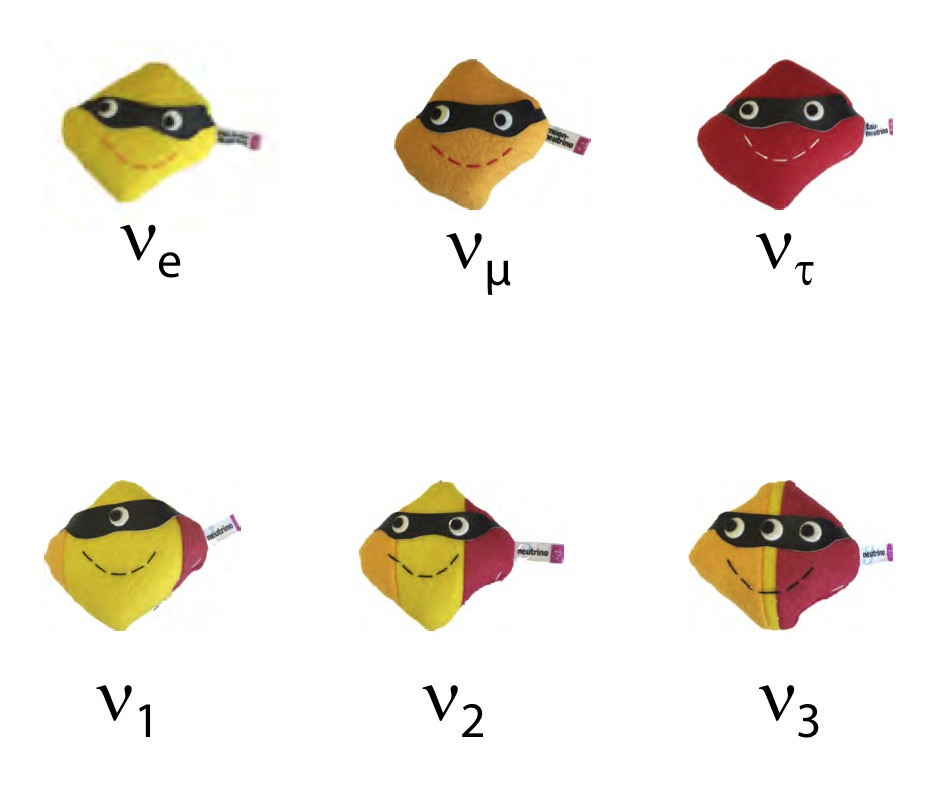
\includegraphics[height=6cm]{graphics/IntroFigures/Fig_01_neutrinos.jpg}
\end{dunefigure}



\begin{dunefigure}
[Electron neutrino appearance signal and background as seen in ArgoNeut]
{fig:Argoneut}
{Electron neutrino appearance signal (top) and background (bottom) as seen in the ArgoNeut experiment\protect{\cite{Acciarri:2016sli}}.  In the true appearance signal, an electron is seen emerging from the primary vertex, then showering.  In the background interaction, a muon neutrino enters and  produces a final-state muon and photons that propagate some distance before showering.}
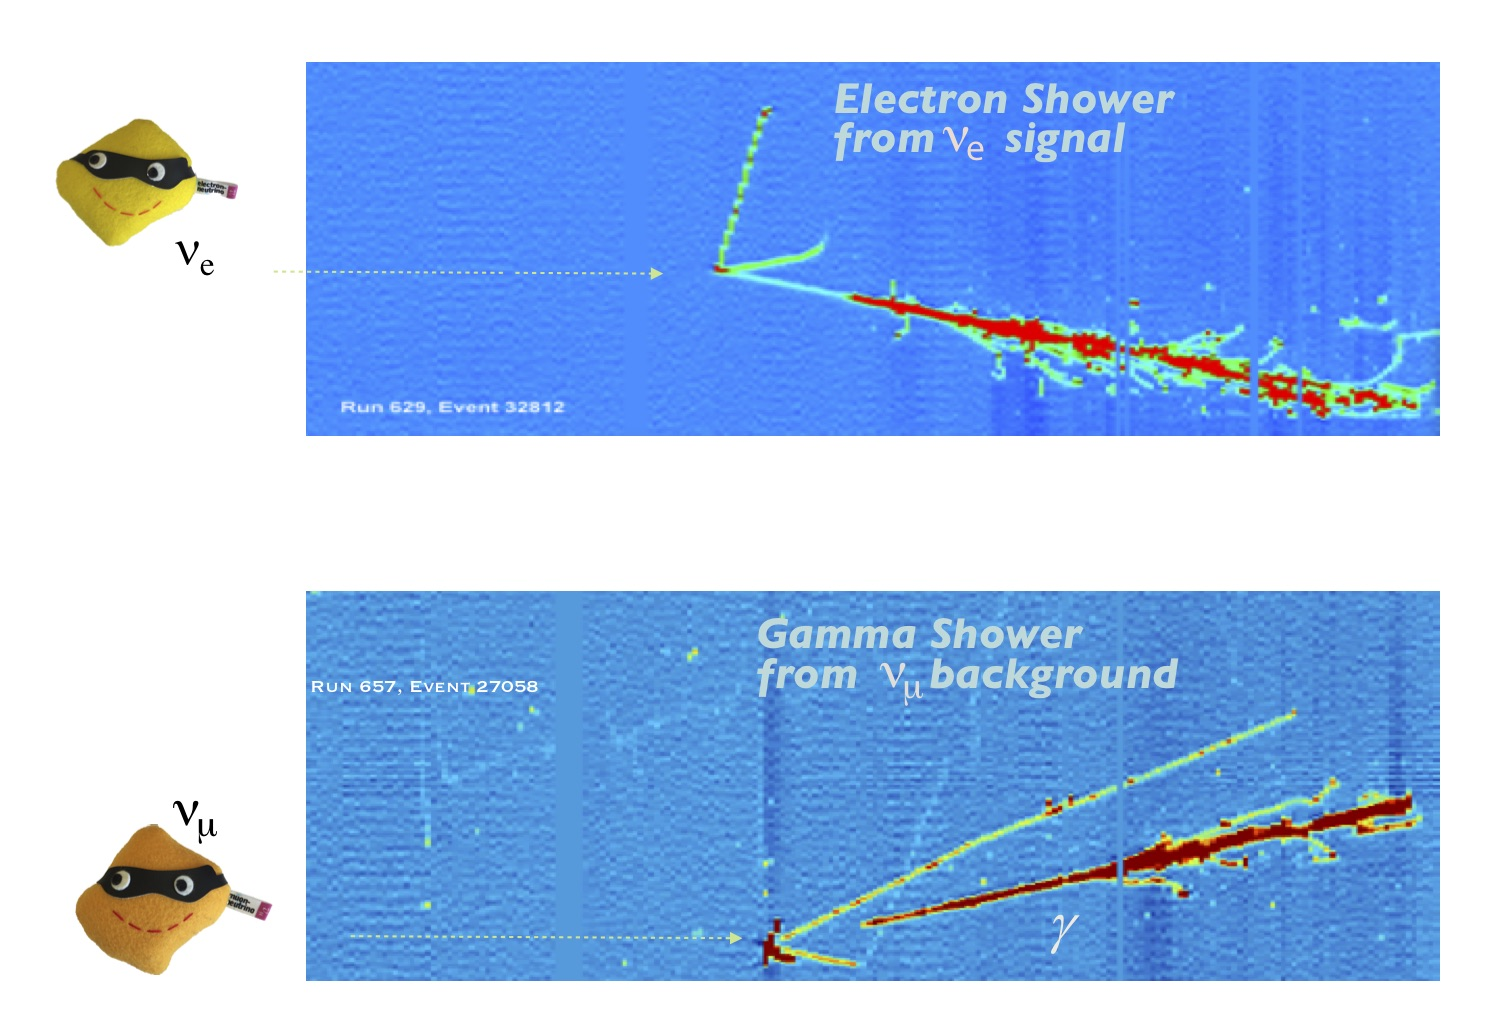
\includegraphics[trim={0cm 0.6cm 2.5cm 0.7cm},clip,height=6cm]{graphics/IntroFigures/Fig_02_Argoneut.jpg} 
\end{dunefigure}


DUNE,  in particular,   wishes to understand the conversion of the muon neutrinos created in Illinois %Anne Illinois 
 into electron neutrinos at the \dword{fd} %in the Homestake mine 
 in South Dakota  %HMS made the change
and compare that conversion rate between neutrino and antineutrino beams. The location of the \dword{fd} and energy of the neutrino beam were chosen to maximize the oscillation effect.   A difference in the conversion rate for neutrinos and antineutrinos could be evidence for matter-antimatter asymmetry in the neutrino sector, a phenomenon called \dword{cpv}.  

To make these measurements, the experiment must be able to distinguish %Anne we need to be able to distinguish %Kirby "we->the experiment"
electron neutrino interactions  from the dominant muon neutrino interactions one would expect in the absence of oscillations.  %Anne Doing t
Doing this requires a very large detector, as neutrino interactions are intrinsically rare, but an extremely  fine-grained one, as well.  Noble liquid  \dwords{tpc}, %time projection detectors, %HSM doesn't \dword{tpc} do that? 
which read out large transparent volumes of liquid by drifting electrons from interactions to charge-sensitive detectors through strong electric fields (\efield{s}), have the needed capabilities of extremely large scale and fine-grained resolution. The proposed DUNE far detector will instrument four \SI{14x12x58}{m} % $14\times12 \times58$ meter 
volumes of \dword{lar} with readout granularity of $\sim$0.5\,cm.  The \dword{fd} modules will be located 4850\,ft below the earth's surface to lower the rate of cosmic rays traversing the detector by orders of magnitude and thus allow sensitivity to very low-energy solar and astrophysical neutrinos, as well as the higher-energy neutrinos produced in the beam at Fermilab.  %Anne at Fermilab.
%Anne - I would reference the FD TDR Vol 1 where there is an excellent discussion of how LArTPC satisfy physics requirements.

Additionally, physics programs focused on nucleon decay, the detection of a \dword{snb}, and other \dword{bsm} signatures take advantage of the large size of the detector and flexible readout window of the \dword{daq} and \dword{lartpc}. %Kirby


The neutrino beam from \dword{fnal} will be pulsed approximately once per second, 24 hours per day during running periods, % anne with 
yielding of order 15 million pulses per year.  Because neutrinos interact  extremely rarely, we expect to detect of order 7,000 neutrino interactions/year in each of the four planned 10\,kt \dwords{detmodule}%Anne located at the \dword{fd} site in South Dakota. 
\footnote{This is based on the beam repetition rate of 0.83\,Hz and an estimated uptime for the accelerator complex of 56\% \cite{Abi:2020evt}.}.


%Anne - I would leave this out Construction of the detector halls and infrastructure for the large 10\,kt fiducial volume \dword{fd} modules is starting now, as are design and construction of detector readout modules.  
A full \dword{tdr} for the first \dword{detmodule}, a horizontal-drift \dword{lartpc},
% Anne program
% anne (it was completed some time ago) has recently been completed and 
is available in References~\cite{DUNE:2020lwj, Abi:2020evt, Abi:2020oxb, Abi:2020loh}.  %anne A  design report for a second detector, using \dword{vd} technology and planned to come online soon after the first \dword{hd} module is being finalized and is included in the computing planning reported here.
 A \dword{cdr} for a second detector module that implements \dword{spvd} is available in Reference~\cite{bib:spvd-cdr-edms}. This module is planned for commissioning soon after the \dword{sphd} module is operational and plans for its computing needs are included in the present document. 
%The  \dword{dune} neutrino oscillation experiment will receive beam late in this decade with commissioning of the \dword{daq} %anne data acquisition 
The first two \dwords{detmodule} should go live late in this decade with commissioning of the \dword{daq} %data acquisition 
systems %for the first %far detector 
%modules 
expected to start in 2027. % anne-28.  We assume the DAQ starts firing up a year early. 

%\todo{CHeck working about the VD I just put in the above paragraph - HMS 3/12}

\begin{dunefigure}
[A far detector cryostat and the horizontal drift \dshort{tpc} structure]
{fig:DUNESchematic} %  HMS doneAnne: label should have fig:
{(Left) A far detector cryostat that houses a 10\,kt \dword{fd} module with horizontal drift technology. The figure of a person indicates the scale.  (Right) A 10\,kt  \dword{dune} \dword{fd} \dword{spmod}, showing the alternating 58\,m long (into the page), 12\,m high anode (A) and cathode (C) planes, as well as the field cage that surrounds the drift regions between the anode and cathode planes. The modular anode and cathode planes are constructed of units called \dwords{apa} and \dwords{cpa}; the blank area on the left side was added to show the profile of a single \dword{apa}.}
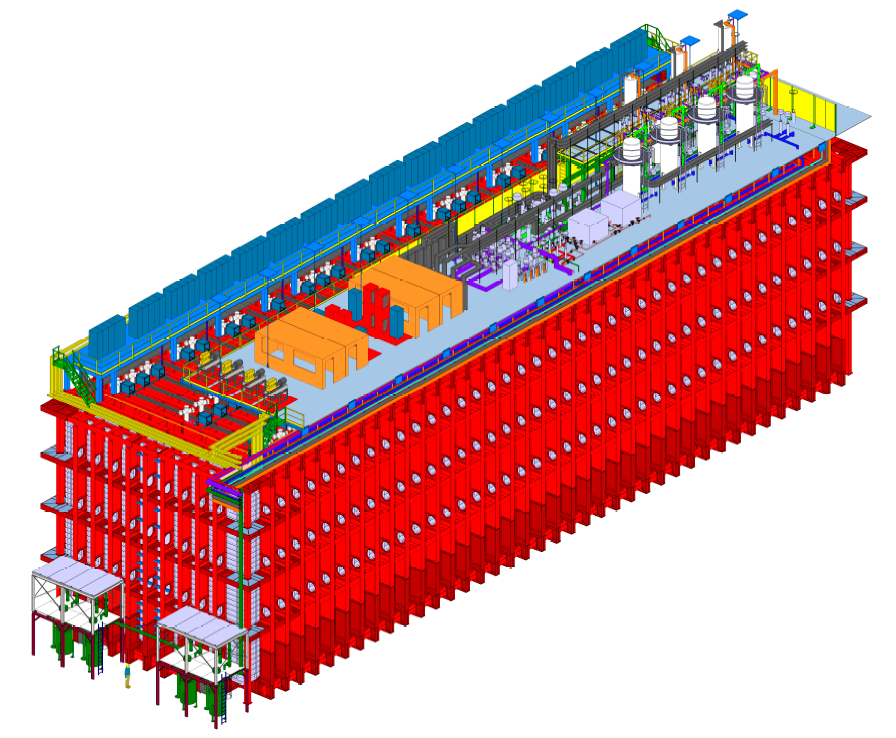
\includegraphics[height=0.35\textwidth]{graphics/IntroFigures/Fig_03a_cryostat-scale.png}
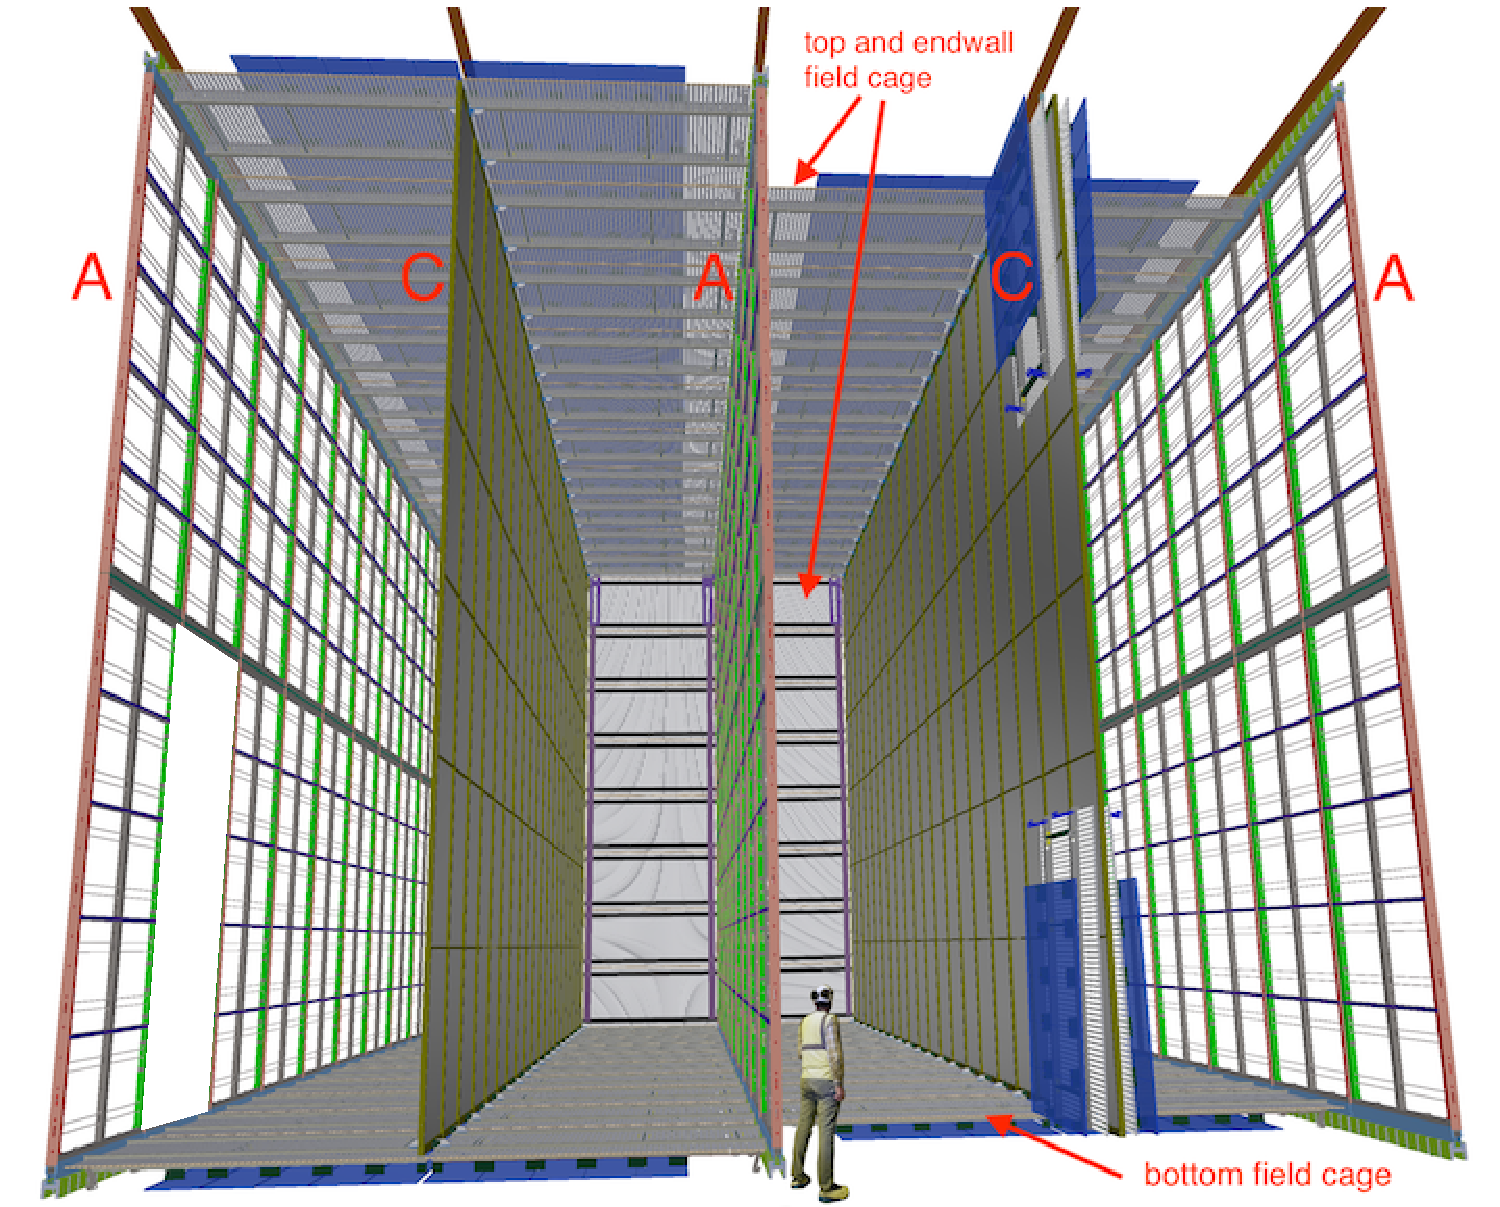
\includegraphics[height=0.35\textwidth]{graphics/IntroFigures/Fig_03b_DUNESchematic.pdf}
\end{dunefigure}


\section{ProtoDUNE Tests at CERN  %anne ProtoDUNE tests at CERN 
\hideme{Schellman/Pennacchio-draft}}

Building an experiment of this size requires an extensive period of prototyping.   The Argoneut\cite{Acciarri:2018myr}, MicroBooNE\cite{microboone} and ICARUS\cite{icarus} collaborations have demonstrated the capabilities of \dwords{lartpc} for neutrino detection on scales between 1 and 500 metric tons (tonnes, t) of fiducial mass.  In preparation for the \dword{dune} experiment, a campaign for testing % anne proposed DUNE 
%st since 1-ton not hypenated inserted the correct plural tons
%HMS - I think this ok now\fixme{st should we have a SI reference to ton--can refer to English or metric (anne) we just use t and kt; I added 'metric' above for clarity}
full-sized \dword{fd} components in 700\,tonne-capacity cryostats %anne detectors 
in the \dword{ehn1} hadronic test beam at the \dword{cern} was launched in 2018.  Both \dword{sp} (horizontal drift) and \dword{dp} (liquid and gas, vertical drift) prototypes, called \dword{pdsp} and \dword{pddp} respectively, were constructed and operated. %anne tested. % Kirby - I like this suggestion so included it with slight addition.
The full data taking chain from detector construction to full offline reconstruction and analysis of data was tested, and the results have yielded considerable insight into the computing challenges for the full \dword{dune} experiment.

\subsection{\dshort{pdsp}} %anne ProtoDUNE Single Phase}
The \dword{pdsp} experiment began taking data %at \dword{cern} 
in late 2018.  \dword{pdsp} %anne uses single-phase technology where 
collects ionization electrons %anne are collected 
directly from the \dword{lar}. The readout system consists of  %anne Anode Plane Assemblies (
\dwords{apa} (APAs).
%anne , which each have 3 layers of wires arranged in different directions. Each layer contains 800-1200  wires spaced 0.5 cm apart. Electrons drift from the original interaction in the Argon, through a strong electric field, to the wire planes and induce signals.  The location in the plane of hit wires gives one coordinate, the time the signal takes to drift to the wire from the original interaction measures a second coordinate.  The third coordinate is derived by combining information from overlaps of signals in the 3 different wire layers.  Signals are amplified electronically and then digitized.  
% anne: From the TDR:
Each \dword{apa} consists of an aluminum frame with three layers of active wires, strung at angles chosen to reduce ambiguities in event reconstruction, that form a grid on each side of the \dword{apa}. The relative voltage between the layers is chosen to ensure transparency of the first two layers ($U$ and $V$) to the drifting electrons. These layers produce bipolar induction signals as the electrons pass through them. The final layer ($X$) collects the drifting electrons, resulting in a unipolar signal. The pattern of ionization collected on the grid of anode wires provides the reconstruction in the remaining two coordinates perpendicular to the drift direction. 
Figure \ref{fig:tpcconcept} illustrates the principle of operation. %anne of a generic \dword{lartpc}.

%% Anne to here 3/14 before moving to ch 7
Horizontal drift \dword{sp} technology with \dword{apa} readout, similar to those used in \dword{pdsp}  will be used for the first of the four \dword{fd} modules. 


\begin{dunefigure}
[Signal formation in a LArTPC with three wire planes]
{fig:tpcconcept} % Anne: label should have fig:
{Diagram  from  \protect{\cite{ Acciarri:2017sde}}  illustrating the signal formation in a \dword{lartpc} with three wire planes~\cite{Acciarri:2016smi}. For simplicity, the signal in the first (U) induction plane is omitted in the illustration. }
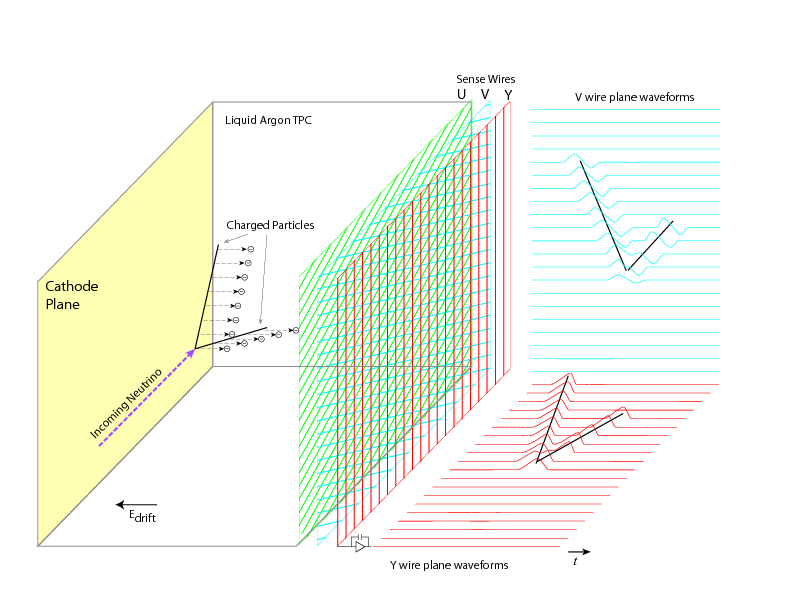
\includegraphics[trim={0cm 0.6cm 2.5cm 0.7cm},clip,height=8cm]{graphics/IntroFigures/Fig_04_LArTPC_Concept.png}
\end{dunefigure}

The \dword{pdsp} detector, immersed in 700\,t of \dword{lar}, consists of %anne a 700 ton volume of liquid argon with 
a cathode plane in the center and sets of three \dwords{apa} mounted side-by-side on %anne each  edge 
either side of the liquid volume, creating %a 
equal and opposite horizontal \efield{}s on the two sides. %The \efield is horizontal so this technology is designated \dword{hd}.   
The maximum drift distance is  3\,m with a nominal voltage of 180\,kV  across that distance.  Each \dword{apa} has 2560 channels and each channel reads out a 12\,bit \dword{adc} every 0.512\,$\mu$sec. %anne  For \dword{pdsp} the readout time appropriate for a 3 m drift was set to 3 msec, 
The appropriate readout time for this configuration was determined to be 3\,ms, resulting in 6000 12\,bit samples per channel per readout window. 
%st fixed \todo{Anne: previous sentence doesn't make sense to me. 6000 per channel per readout window?}
%ST changed 3 s to 3 ms on the readout time. 0.5 microseconds * 6000 = 3 milliseconds
The total data size for six \dwords{apa} is thus 140\,MB with additional header and data from photon and external tagging systems, bringing the nominal \dword{tr} size up to about 180\,MB.  Lossless compression of the \dword{tpc} readout data was implemented in the \dword{daq}, resulting in a final compressed event size of about 75\,MB. 


%\subsubsection{Trigger Records \hideme{draft}}

Neutrino experiments, and in particular \dword{tpc}-based experiments, may or may not have internal triggers but they are generally read out over a fixed time window.  For \dword{protodune}, \dword{microboone}, \dword{minerva} and the \dword{minos} and \dword{nova} near detectors, a readout generally corresponds to either the 10\,$\mu$sec beam spill or a multi-msec \dword{tpc} drift time.  Within that time span, multiple beam, cosmic ray or rock muon interactions may occur within the active detector volume.  Thus the unit of detector readout, the \dword{tr}, does not correspond directly to a single interesting interaction, but to a group of interactions. The processing frameworks that we use have grown out of collider experiments and are based on the concept of an ``event,'' generally a beam crossing, that is processed as a unit.  DUNE prefers to use the term ``trigger record'' rather than ``event'' for the unit of processing, as it avoids confusion between an interaction ``event'' and a readout ``event.''  


The test beam ran at rates of up to 25\,Hz over a period of six weeks at beam momenta between 0.5 and 7\,GeV/c.  Time-of-flight and Cherenkov counters in the beamline provided beam flavor tagging.  Around 8M total ``physics'' records were written, with around 3M having beam tag information.  In total  850\,TB of raw test beam data were written, along with one PB of commissioning and cosmic data. These data were successfully cataloged and written to storage at both \dword{cern} and \dword{fnal} at rates of up to 2\,GB/sec.   

Thanks to significant prior effort in the \dword{lartpc} %Kirby fixed \todo{Anne:is it really \dword{lartpc}?}
computing and algorithms community, reconstruction software was ready to go. The first reconstruction pass began soon after data taking started and was complete within two weeks of the end of data taking.  These results were extremely useful in demonstrating the capabilities of the detector; they are summarized in Volume II of the \dword{sphd} \dword{tdr}~\cite{Abi:2020evt}.  A second pass, with improved treatment of instrumental effects ranging from stuck bits, to \twod deconvolution, to correction for space charge effects, was completed in late 2019. Another pass with major improvements to the electrostatic modeling and reconstruction algorithms was launched in 2021. 

%\dword{pdsp} Reconstruction - from raw data to beam interactions and cosmics full reconstructed with 80-90\% efficiency - has been performed twice over the 8M interactions recorded during the test-beam runs. 
Figure~\ref{deconvolution} illustrates the signal processing stage of reconstruction, where raw \dword{adc} signals have noise and stuck bits removed and are then deconvoluted to yield Gaussian hit candidates. An important aspect of the reconstruction of APA-based \dword{lartpc}s is the need for a 2D signal processing and deconvolution to include extending the time domain beyond the interaction timing window to account for \dword{fft} edge effects. The impacts the reconstruction algorithms and framework processing. Figures~\ref{wire-cell-bee} and~\ref{pandora} illustrate full pattern recognition and event reconstruction. 

While \dwords{lartpc} benefit from fine granularity and a uniform detector medium, it is possible for diffusion, argon purity variations, fluid flow and the build up of space charge in the active medium %anne can all 
to introduce distortions into the detector response.  These effects have all been simulated and tested in the \dword{pdsp} data. 

Compressed raw input trigger records were of order 75\,MB in size and took 500-600 seconds to reconstruct, of which around 180\,s was signal processing and the remainder high-level reconstruction dominated by 40-60 cosmic rays per readout.  Memory footprints for data processing ranged between 2.5 and 4\,GB.  Output   record sizes were reduced to 35\,MB by dropping the raw waveforms after hit finding.   Data reconstruction campaigns took of order 4-6 weeks (similar to the original data taking) and utilized up to 15,000 cores on \dword{osg} and \dword{wlcg} resources.  Job submission was done through the \dword{poms}\cite{poms} job management system developed at \dword{fnal}. \dword{poms} supports submissions to \dword{fnal}-dedicated resources and selected \dword{osg} and \dword{wlcg} sites.  Figure \ref{sites} shows the distribution of wall hours used for reconstruction in 2019.
These metrics have influenced the ideas regarding memory utilization, event data model, and workload/workflow management in this document.

For reconstruction, data were streamed via {\tt xrootd}\cite{Behrmann:2011zz} from \dword{dcache} storage at \dword{fnal} to the remote sites. Despite individual processing jobs taking 15-30 hours to complete, network interruptions rarely caused job failures. 


\begin{dunefigure}
[Raw and deconvolved induction U-plane signals before and after signal processing]
{deconvolution} % Anne: label should have fig:
{Comparison of raw (left) and deconvolved induction U-plane signals (right) before and after 
the signal processing procedure from a \dword{pdsp} \dword{tr}. The bipolar shape with red (blue) color representing
positive (negative) signals is converted to the unipolar shape after the \twod deconvolution.}
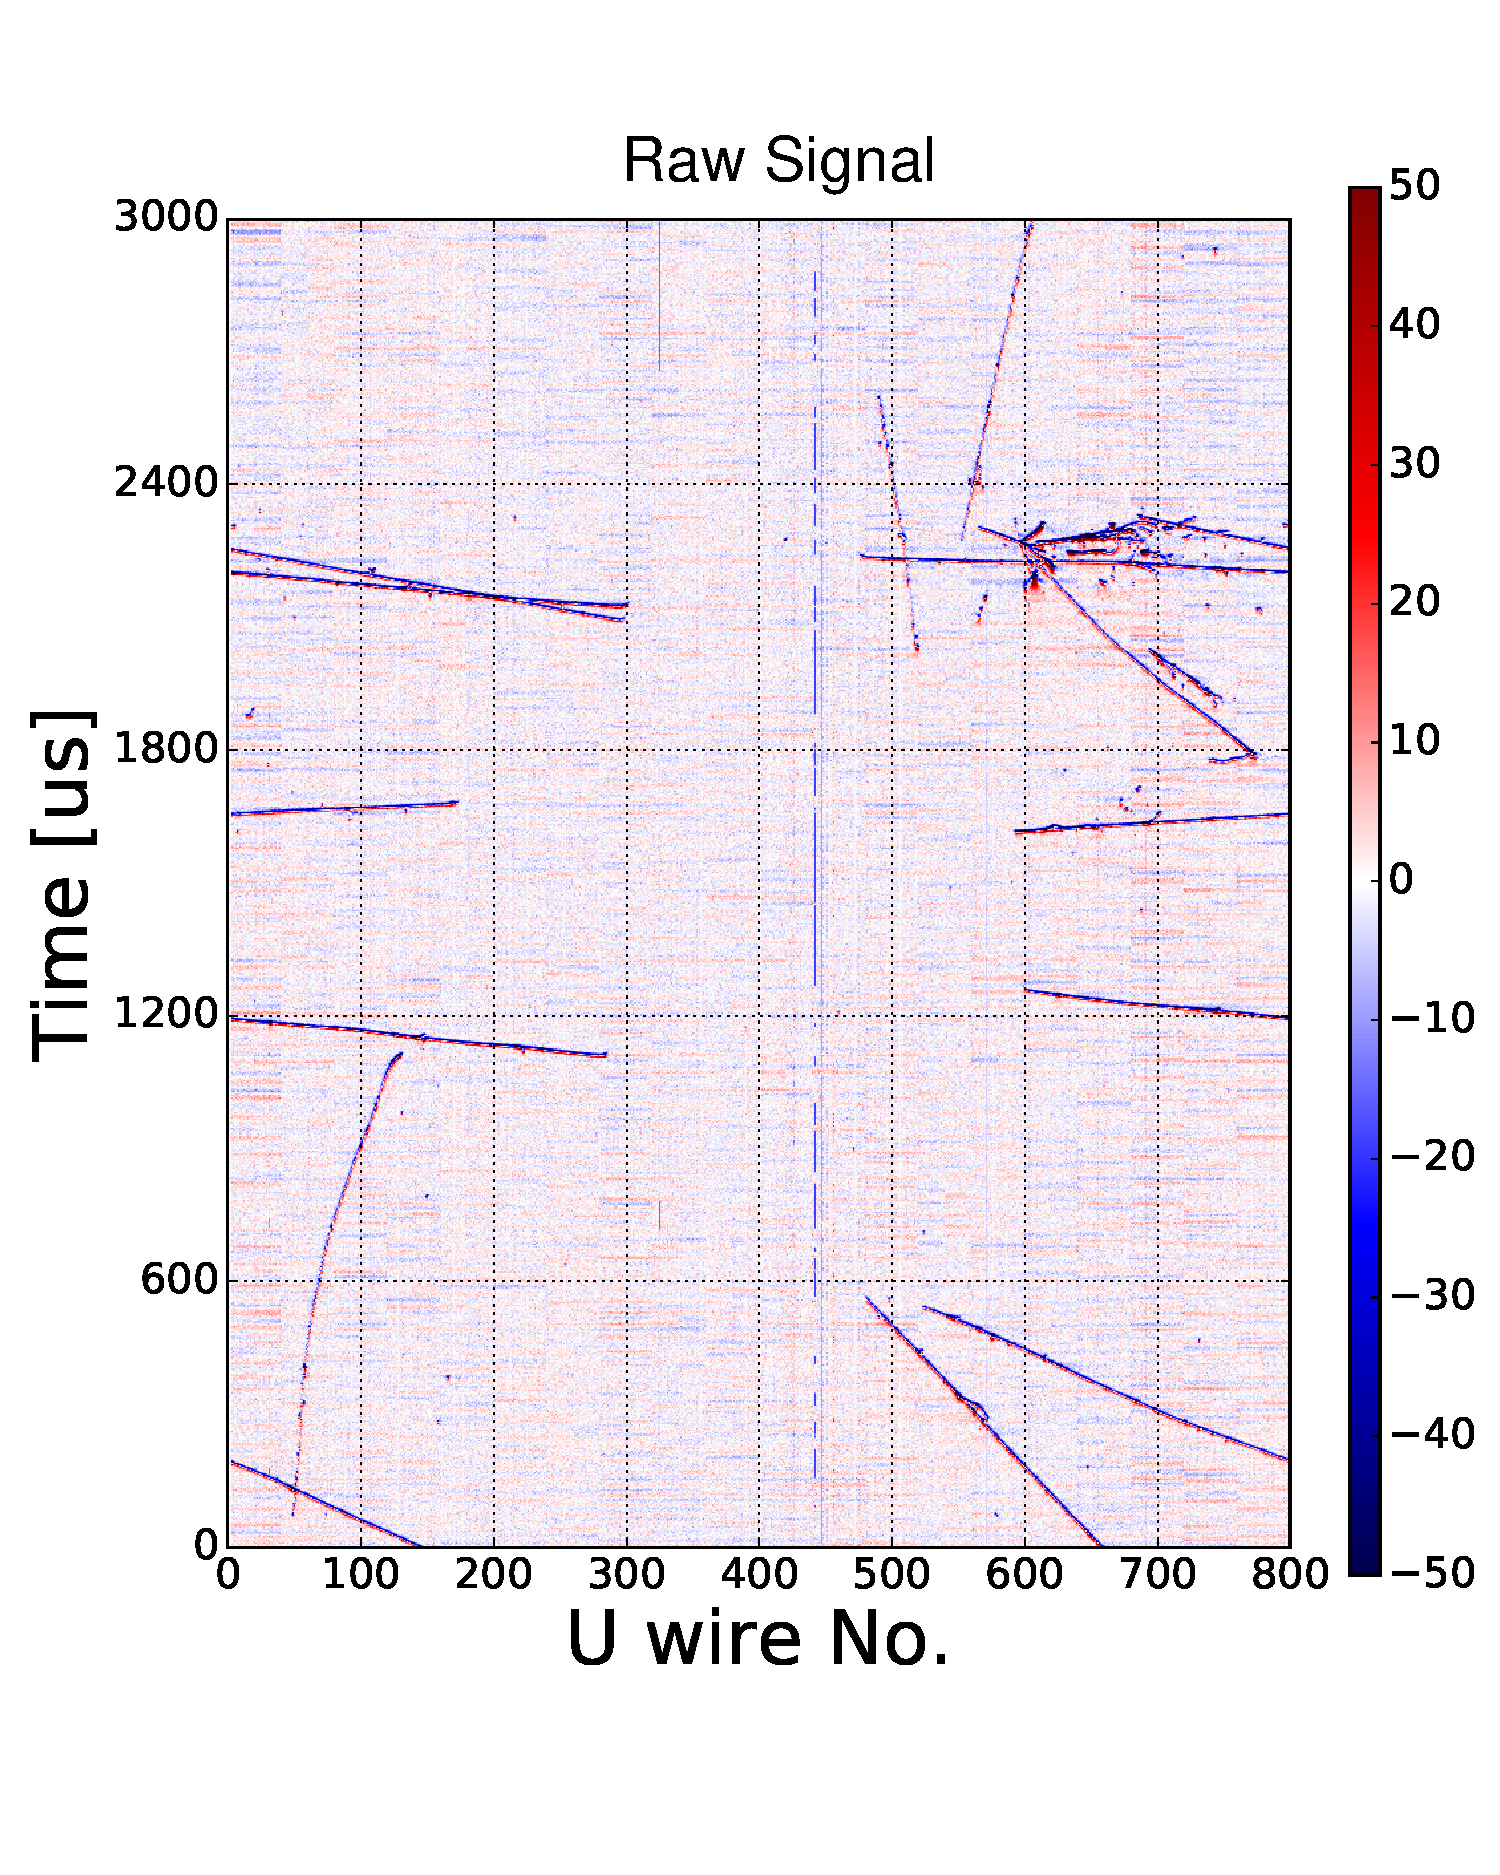
\includegraphics[width=0.49\textwidth]{graphics/IntroFigures/Fig_05a_protodune_raw_u.pdf}
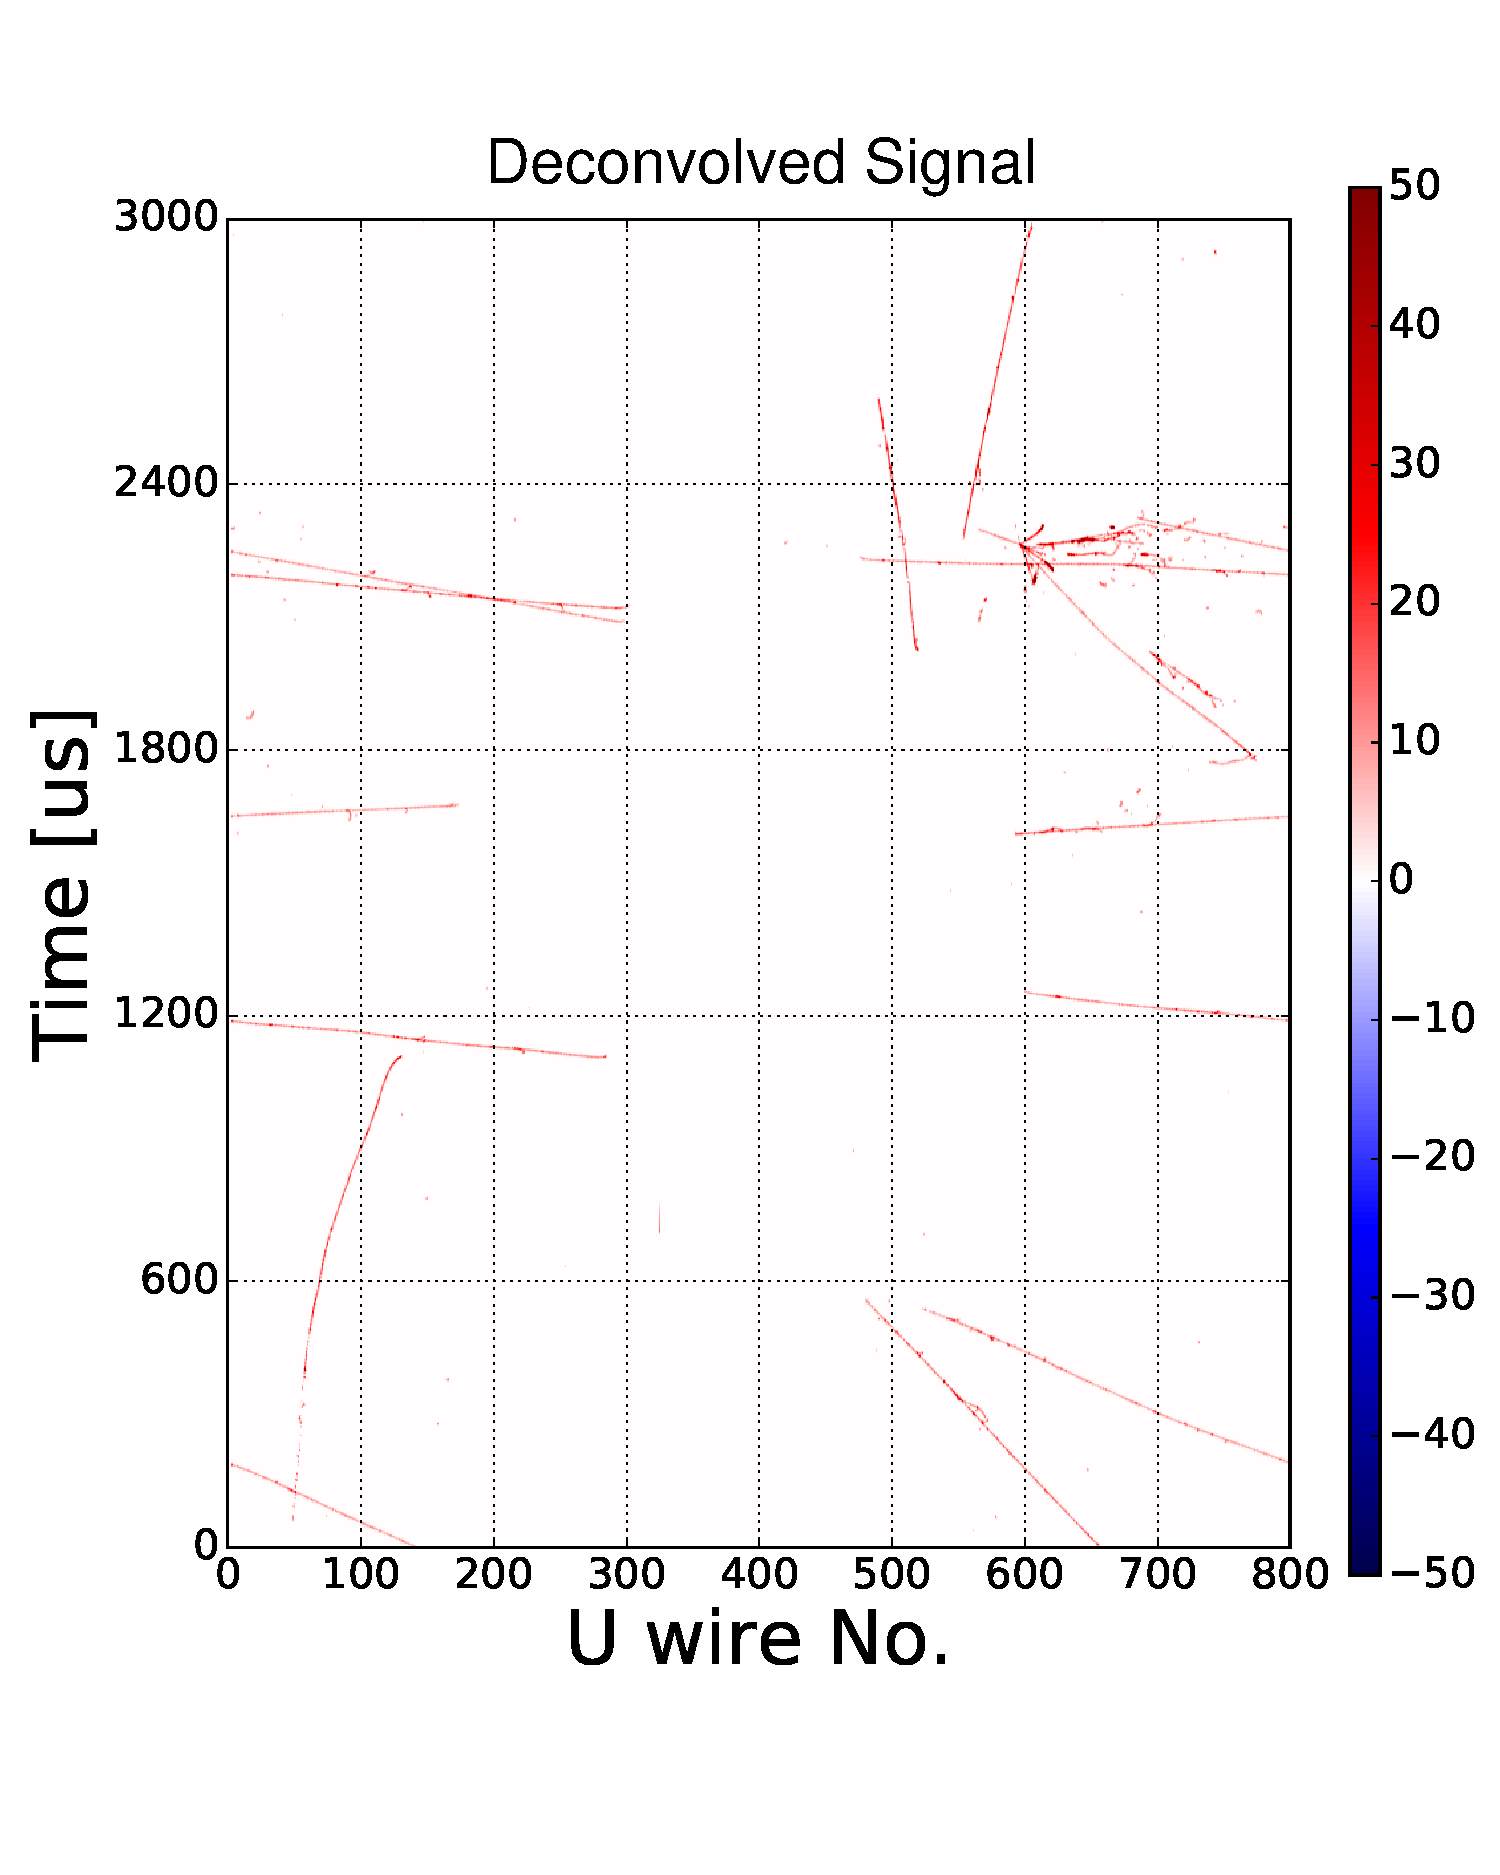
\includegraphics[width=0.49\textwidth]{graphics/IntroFigures/Fig_05b_protodune_decon_u.pdf}
\end{dunefigure}

\begin{dunefigure}
[Cosmic rays and beam interaction in \dshort{pdsp}]
{wire-cell-bee} % Anne: label should have fig:
{The \dword{pdsp} detector (gray box) showing 
the direction of the particle beam (yellow line on the very far left) and the outlines of the six \dwords{apa}. Cosmic rays
can be seen throughout the white box, while the red box highlights the beam region of interest with an interaction of the 7\,GeV beam. 
The \threed points are obtained using the Space~Point~Solver reconstruction algorithm.}
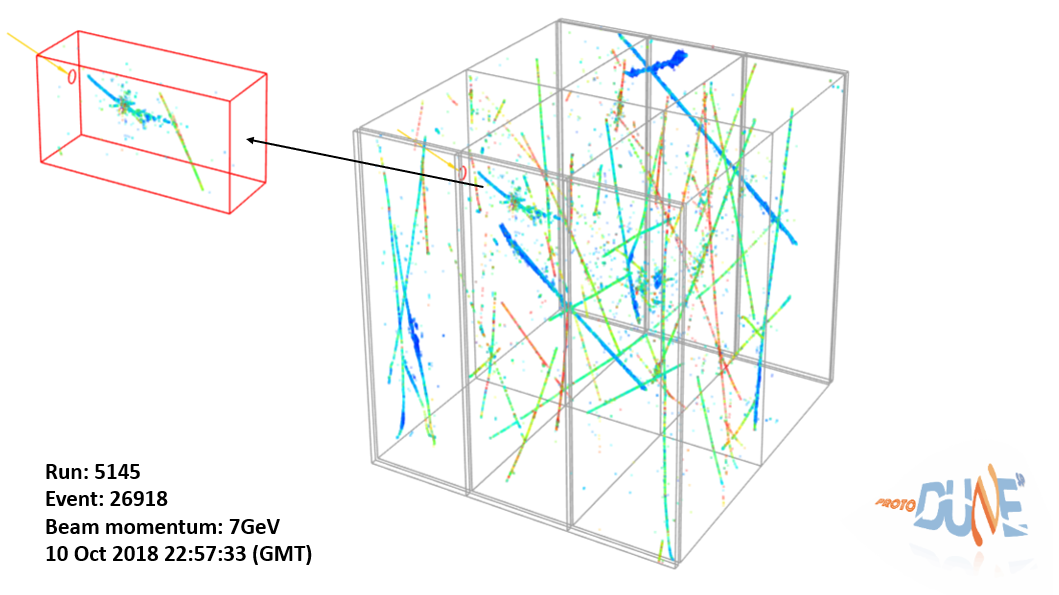
\includegraphics[width=0.9\textwidth]{graphics/IntroFigures/Fig_06_bee_event.png}
\end{dunefigure}


\begin{dunefigure}
[Pandora reconstruction of cosmic rays and beam interaction in a \dword{pdsp} trigger record]
{pandora}
{Pandora \protect{\cite{Acciarri:2017hat}} reconstruction of cosmic rays and beam interaction in a \dword{pdsp} \dword{tr}. The left side of the figure shows the full detector volume with all interactions, including cosmic rays and the right side shows the identified beam interaction.}
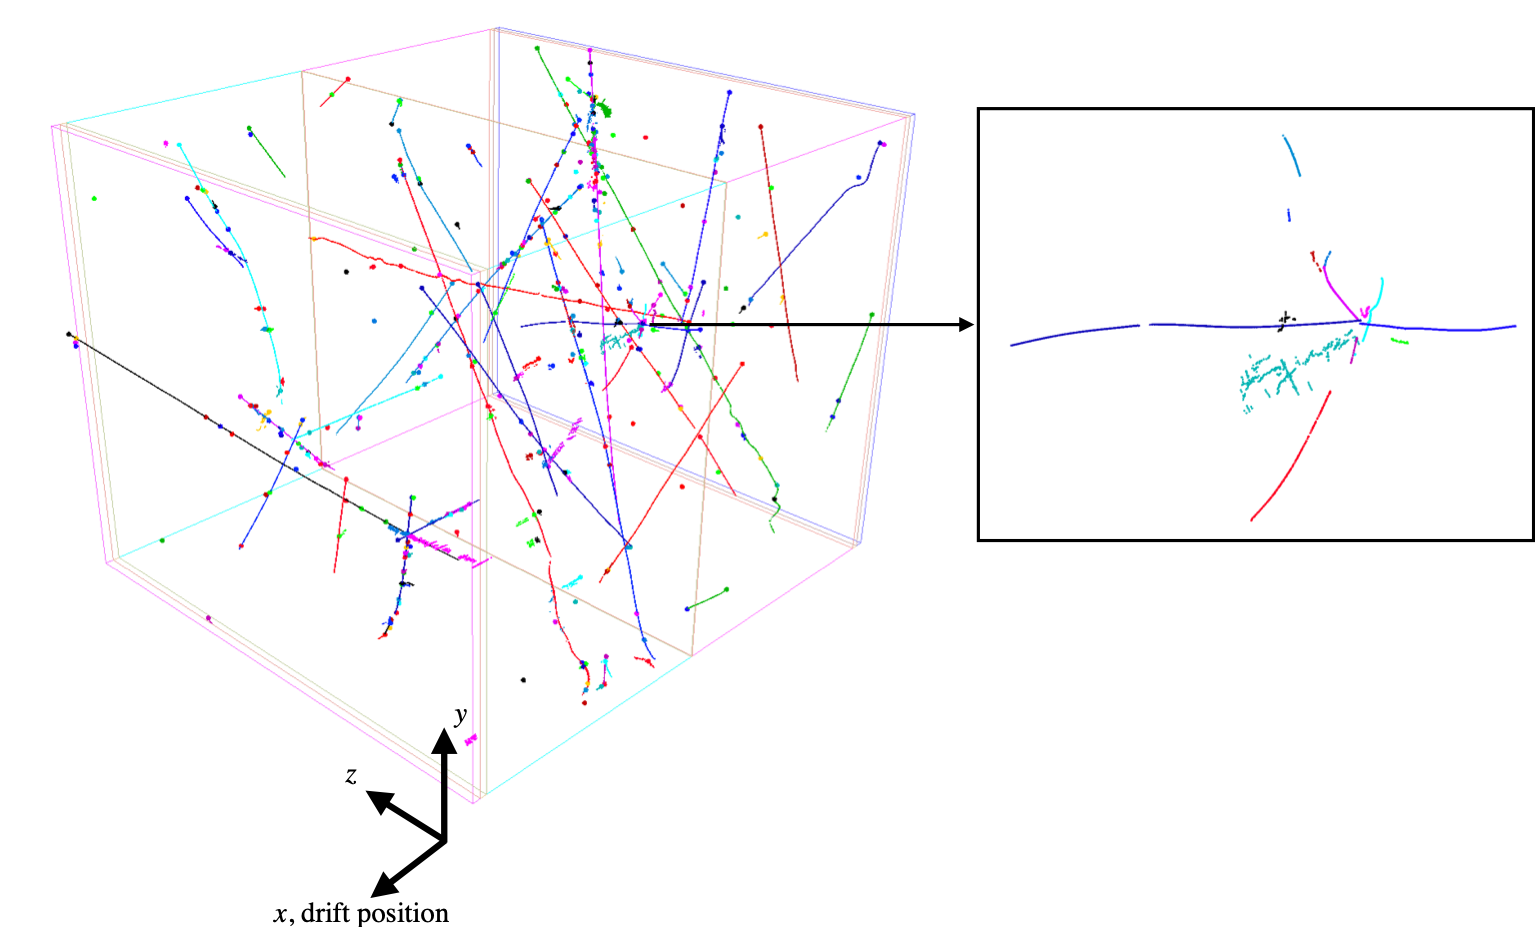
\includegraphics[width=0.8\textwidth]{graphics/IntroFigures/Fig_07_pandora.png}
\end{dunefigure}


\begin{dunefigure}
[Reco/sim processing distribution across sites for DUNE production, 2019]
{sites} % Anne: label should have fig:
{Reconstruction and simulation processing distribution across sites for DUNE production in calendar 2019.  The inner circle shows national contributions while the outer circle shows individual site contributions.}
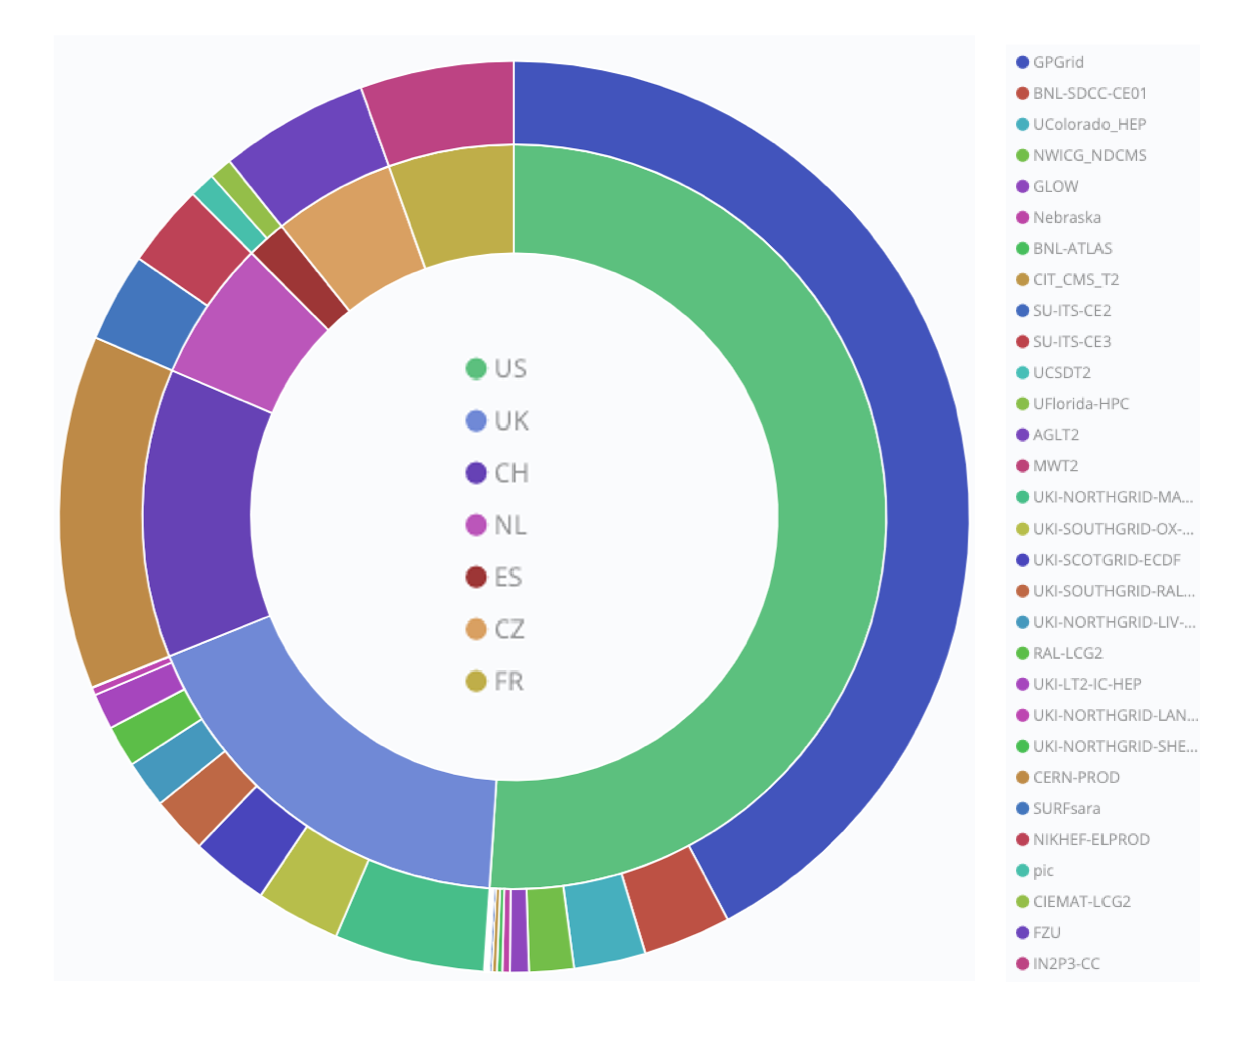
\includegraphics[height=0.65\textwidth]{graphics/IntroFigures/Fig_8.pdf}
\end{dunefigure}

\subsection{ProtoDUNE Dual-Phase and its Evolution to the Vertical Drift Design \hideme{Pennacchio - draft}}
%anne to start here monday

%The \dword{pddp} detector began taking data using cosmic rays in August 2019.  Thanks to preceding data challenges, those data have been successfully integrated into the full data cataloging and reconstruction chains and are now being reconstructed as they arrive.   The \dword{pddp} technology locates the readout systems above a thin layer of argon gas above the liquid argon surface.  This gas layer allows an external electric field to accelerate the electrons and produce gas amplification.  The result is a substantial increase in signal-to-noise in the resulting signals, at the cost of longer electron drifts from the bottom of the liquid volume.  Figure \ref{dpevent} illustrates early data from \dword{pddp}. 

In parallel with the single-phase horizontal-drift detector tests, a vertical drift  \dword{dp} readout prototype (\dword{pddp})
in a similar cryostat was also  tested.  \dword{pddp} was not exposed to beam but ran on cosmics in 2019 and 2020. 

The basic operating principle of \dword{pddp} is shown in Figure~\ref{dp_principle}. Charged particles that traverse the active volume of the \dword{lartpc} ionize the medium while also producing scintillation
light. The ionization electrons drift vertically upward %anne in the vertical direction 
toward an extraction grid just below the liquid-vapor interface. 
After reaching the grid,
an \efield stronger than the drift field extracts the electrons from the liquid up into the gas phase.
Once in the gas, electrons encounter micro-pattern gas detectors, called \dwords{lem}, with high-field regions. The \dwords{lem} amplify the electrons in avalanches that occur in these
high-field regions. The amplified charge is then collected and recorded on a \twod anode consisting
of two sets of 3.125\,mm pitch gold-plated copper strips that provide the $x$ and $y$ coordinates (and
thus two views) of an interaction.   

\begin{dunefigure}
[Principle of \dshort{dp} readout and parameters for extraction]
{dp_principle} % Anne: label should have fig:
{Principle of \dword{dp} readout (left), and thicknesses and HV values for electron extraction from liquid to gaseous argon, their
multiplication by \dwords{lem}, and their collection on the x and y readout anode plane (right) The HV values are
indicated for a drift field of 0.5\,kV/cm in LAr.}
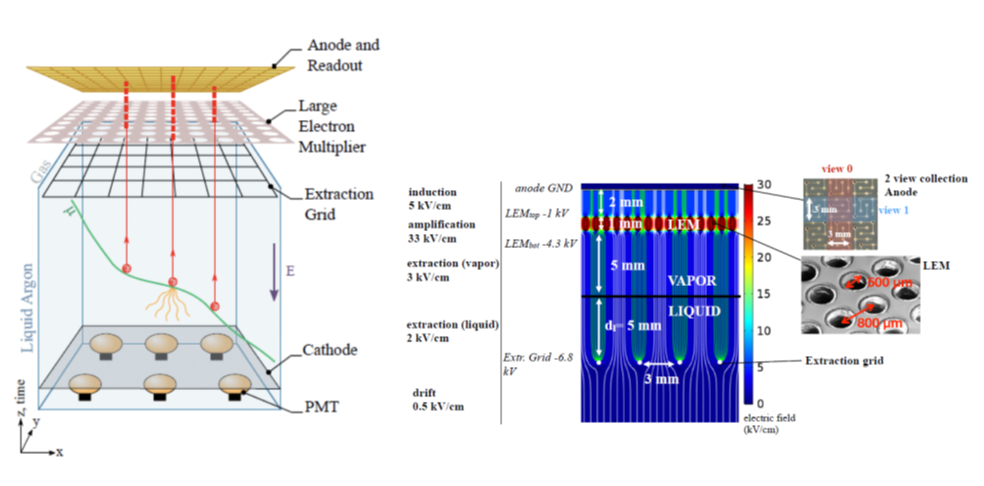
\includegraphics[width=0.85\textwidth]{graphics/IntroFigures/Fig_11_protodune-dp-principle.png}
\end{dunefigure}

The readout area surface is \SI{6x6}{m}, subdivided into four $3\times3$ m$^2$  \dwords{crp}. Each \dword{crp} is an independent detector element %anne insuring 
that performs electron extraction, amplification, and collection. 
The 7680 readout channels are read by   12\,bit \dwords{adc} every 0.4\,$\mu$sec. 
The \dword{pddp} detector   consists of a 700\,t volume of \dword{lar}, with  a vertical drift length of 6\,m, corresponding to a full drift window of 4\,ms (10,000 samples).


The \dword{pddp} detector began taking cosmic ray data in August 2019. Thanks to preceding data challenges, these data have been successfully integrated into the full data cataloguing and reconstruction chain and were   reconstructed as they become available.
A total of 1.45M \dwords{tr} were collected; the size of the raw data files (run sequence files) was 3.2 \,GB, each file containing 30 \dwords{tr}. Cosmic ray data are displayed in Figure~\ref{dpevent}: on
the left a horizontal muon track is shown with the corresponding waveform on a channel, giving an
idea of the low noise conditions. A \dword{tr} including an electromagnetic shower and two muon decays
and a \dword{tr} with an example of multiple hadronic interactions in a shower are shown on the right.

%samweb list-files "data_tier raw and run_type protodune-dp " --summary
%File count:	143583
%Total size:	334,415,580,215,147
%Event count:	1454065

 
\begin{dunefigure}
[Cosmic ray data from \dshort{pddp}]
{dpevent} % Anne: label should have fig:
{Cosmic ray data from the \dword{dp} prototype, \dword{pddp}.}
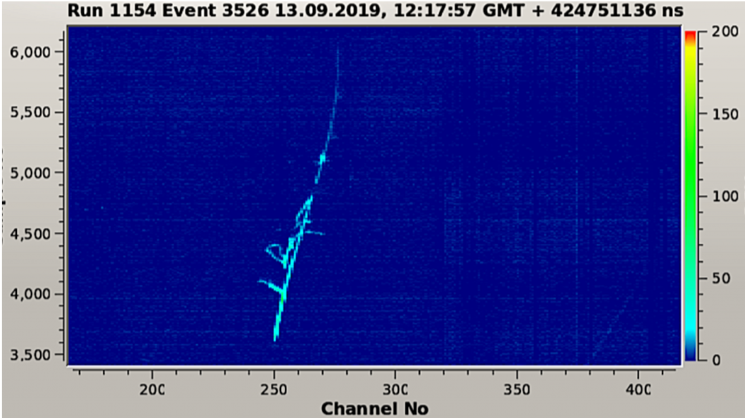
\includegraphics[width=0.85\textwidth]{graphics/IntroFigures/Fig_09_protodune-dp-event.png}
\end{dunefigure}


All data ($\sim$\,330\,TB) taken during different campaigns   have been copied to \dword{fnal}. A subsample is composed of data sets taken during detector transient conditions, motivated by various specific testing needs;  all cosmic ray data taken in well defined and stable detector conditions in 2019 and 2020 ($\approx$\,377K events) have been processed with \dword{larsoft} by performing the reconstruction of hits and \twod tracks. A second pass, including \dword{pandora} reconstruction algorithms, started in spring 2021. 
The memory footprint is between 1.9 and 2.5\,GB
Data management and job submission was successfully done through the same systems as \dword{pdsp}.

In the fall 2020 the \dword{dp} design evolved to the \dword{spvd} concept. The \dword{spvd} incorporates many of the design aspects developed for the \dword{dp}, such as the \dwords{crp};   the  main  difference  with  respect  to  the  \dword{dp}  design  is   the  removal  of  the  extraction  stage  to  the  gas  phase  and  the  subsequent  charge  amplification  stage.  %anne  This  change eliminates the grid immersed in the liquid and biased at high voltage in order to define the field needed to transfer the electrons from the liquid to the gas phase and the \dwords{lem} used to amplify the signal.
This eliminates the grid biased at high voltage (to transfer the electrons from the liquid to the gas) and the \dwords{lem} used to amplify the signal in the gas. The \dword{spvd} \dwords{crp} %anne keeps the concept of charge readout performed 
perform charge readout using %anne with  strips implemented on segmented 
perforated \dword{pcb} anodes with finely segmented strip electrodes %anne while replacing the \dword{lem} micro-pattern detectors, which operated in the argon gas phase and coupled to the anode printed circuit boards with charge collection strips, with perforated anodes 
that are immersed in the \dword{lar}.
 

\begin{dunefigure}
[Vertical drift solution with \dshort{pcb}-based charge readout]
{fig:vd_principle}
{Vertical drift solution with \dword{pcb}-based charge readout}
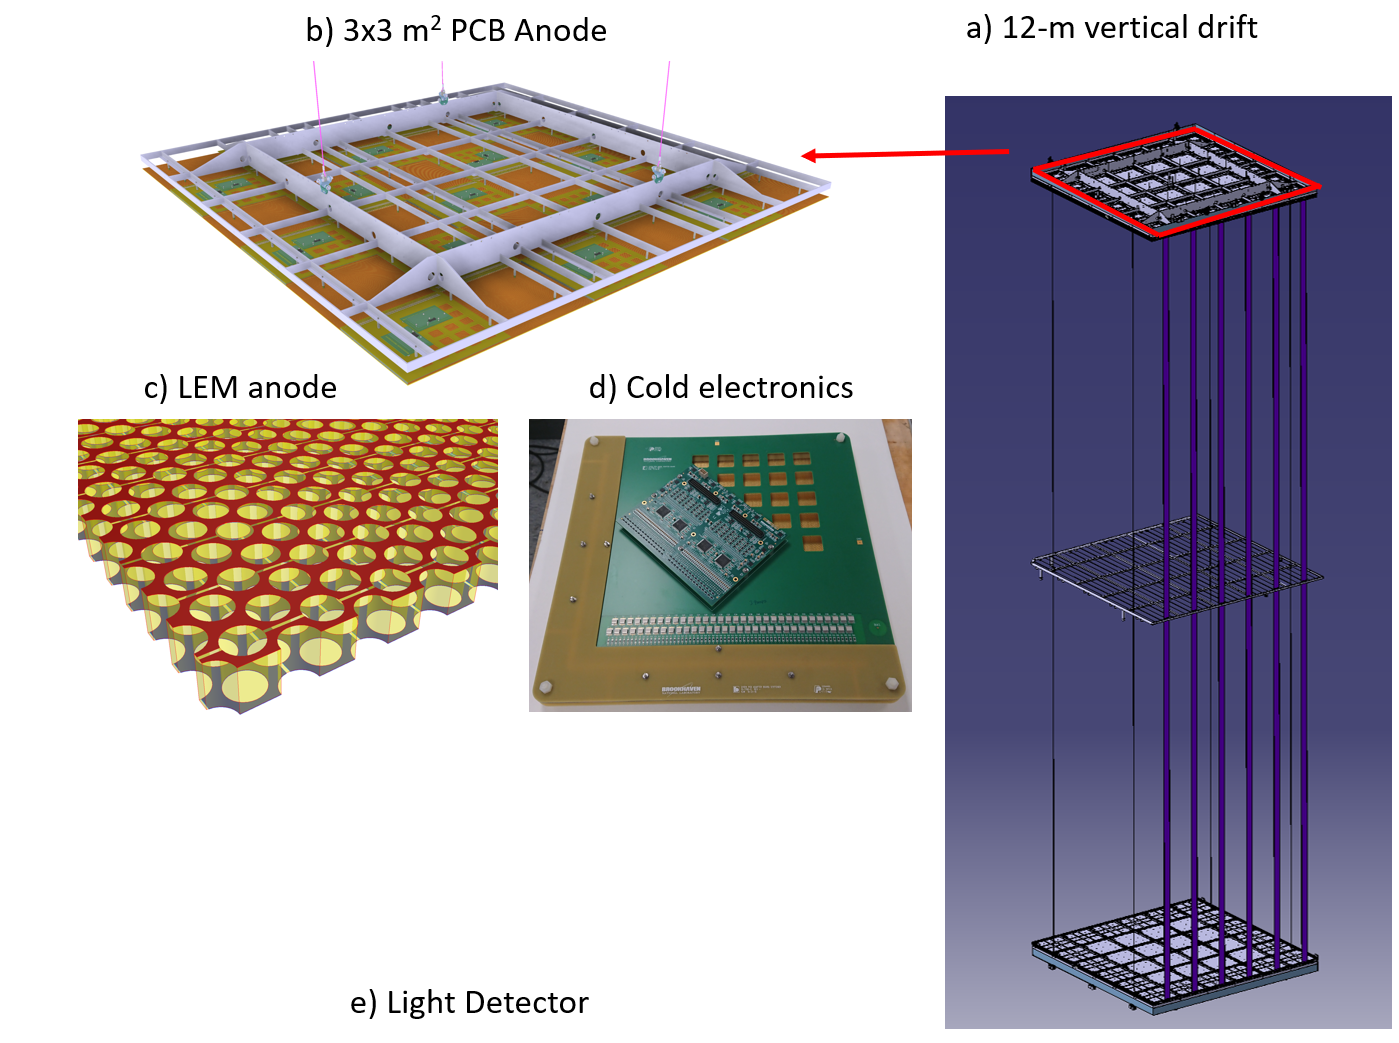
\includegraphics[width=0.85\textwidth]{graphics/IntroFigures/Fig_13_VD_solution.png}
\end{dunefigure}

 Figure \ref{fig:vd_principle} illustrates the \dword{pcb}-based charge readout concept for the \dword{fdvd}. The electron drift direction is vertical.
Two separate drift volumes of 6.5\,m are defined by a cathode plane at roughly mid-height in the
detector volume. Ionization electrons above the cathode will drift upwards; ionization electrons in the liquid below the cathode will drift downwards.
The \dword{spvd}  prototype components have undergone testing starting in 2021 with a small \coldbox; some examples of cosmics tracks are shown in figure \ref{fig:VD_coldbox_trks}. A full prototype, known as \dword{mod0}, is expected to be completed and  installed 
 inside the \dword{np02} cryostat in 2022 and 2023. Long-term operation and full characterization with a charged particle beam will follow. 

\begin{dunefigure}
[cosmic tracks collected during Vertical drift cold box data taking]
{fig:VD_coldbox_trks}
{Examples of cosmic tracks in the Vertical Drift cold box}
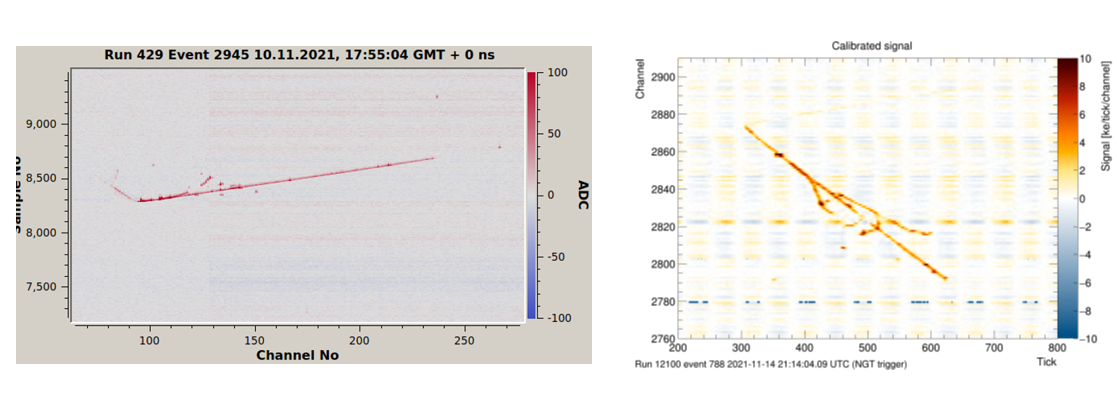
\includegraphics[width=0.85\textwidth]{graphics/IntroFigures/Fig_14_VD_coldbox.png}
\end{dunefigure}


\subsection{Conclusions from Prototype Tests \hideme{Schellman draft}}

\dword{protodune} %anne prototype 
runs are ongoing and will continue through beam tests in 2022-23 at \dword{cern}.  Data cataloging, movement and storage techniques were tested before the start of the \dword{pdhd} and \dword{pdvd}  runs and were able to handle the full rate of the experiments.   Reconstruction algorithms were also in place on time and %anne were able to 
produced early results that led to increased understanding of the detector and improved calibrations for a second iteration.  These tests also identified some deficiencies in our infrastructure, including incomplete schemes for the transmission of configuration and conditions information between hardware operations and  offline computing.  The test beam runs have been extremely valuable in allowing us to determine which variables are important to transmit and in designing improved systems for gathering and storing that information. 

An additional beam run of  \dword{pdsp} is planned for 2022-23, with a cosmic test of the \dword{spvd} design to follow in 2023-24, allowing further development and testing of our computing infrastructure before the full detector comes online in the late 2020s. 

%\section{ProtoDUNE Simulation} % anne discussion 
%\hideme{Yang-needed}

\section{Far Detector %On to Full DUNE 
\hideme{Schellma-draft}}
\label{sec:intro-fd}

The full DUNE \dword{fd} will begin with one \dword{sphd} module to be installed  at \dword{surf} %anne at Homestake 
starting near the end of  this decade.  A second \dword{spvd} module will be installed and commissioned in parallel.  High-intensity neutrino and antineutrino beams should arrive after a year or so of commissioning of the detector and \dword{lbnf} beamline.  The first %anne \dword{hd} 
module will %anne largely resemble 
be a scaled up version of \dword{pdsp} with 150 \dwords{apa} distributed 2-deep %anne 2-deep? at 
the length of the cryostat, down the center and along the long walls. %\anne edges of the cryostat.   
The argon volume will be $15\times14\times62$\,m$^3$ with a total (fiducial) mass of 17\,kt (10\,kt).  Section~\ref{sec:est:FD} summarizes the expected event rates and data volumes for the first two modules.  Two additional detector modules, possibly with updated or novel technologies %anne, beyond the first two 
will be added later. For now, we assume that data volumes and rates coming from other technologies will not exceed %anne be less than or equal to the single-phase values. 
the values for the \dword{sphd} or \dword{spvd}.


%st fix the misprinted sim.. but is of order and sim redundant?

The detector should be sensitive to neutrino interactions and radioactive decays above an energy threshold of order $\sim 5$\,MeV.  Unambiguous triggering may require a somewhat higher threshold  to avoid false triggers due to $^{39}$Ar decays,  but beam interactions in the 500-10,000\,MeV range should have almost perfect detection efficiency. Sophisticated triggering algorithms should also allow standalone detection of astrophysical sources, including higher-energy solar neutrinos and \dword{snb} candidates. 

The data rates will be dominated by 4,500 cosmic rays expected per module/day.  These events are vital for monitoring and aligning the detector. %anne aligning? ST yes we measure to be sure that the APA are in line
The next most significant source of events will be calibration campaigns with radioactive and neutron sources and lasers.  In all cases, the goal is to gather data from the full volume of the detector with as fine a granularity as possible. 

Beam interactions themselves are expected to be quite rare, occurring in only 1/2000 of beam gates ($\simeq$\,2/hr)  Extraction of oscillation parameters will require both powerful electron background rejection, discussed in the previous section,  and precise calibration of the energy scale of the experiment, hence the much larger calibration samples.

Beam, cosmic ray and solar neutrino interactions are reasonably localized in time and space, involving a small fraction of a module over a few milliseconds.  This can, in principle, allow significant reduction in data size without loss of physics information if suitable triggers are used.



\subsection{Supernova candidates \hideme{Schellma -updated early march }}\label{sec:supernova}



\begin{dunefigure}
[Supernova interactions in the FD]
{fig:SNe} % Anne: label should have fig:
{
 Simulated $\nu_e$
 CC event with a 20.25$~sim$ MeV neutrino), showing an electron track and ``blips" from Compton-scattered gammas. The vertical dimension indicates time and the horizontal dimension indicates wire number. Color represents charge. The top panel shows the collection plane and the bottom panels show induction planes. The boxes represent reconstructed hits. }
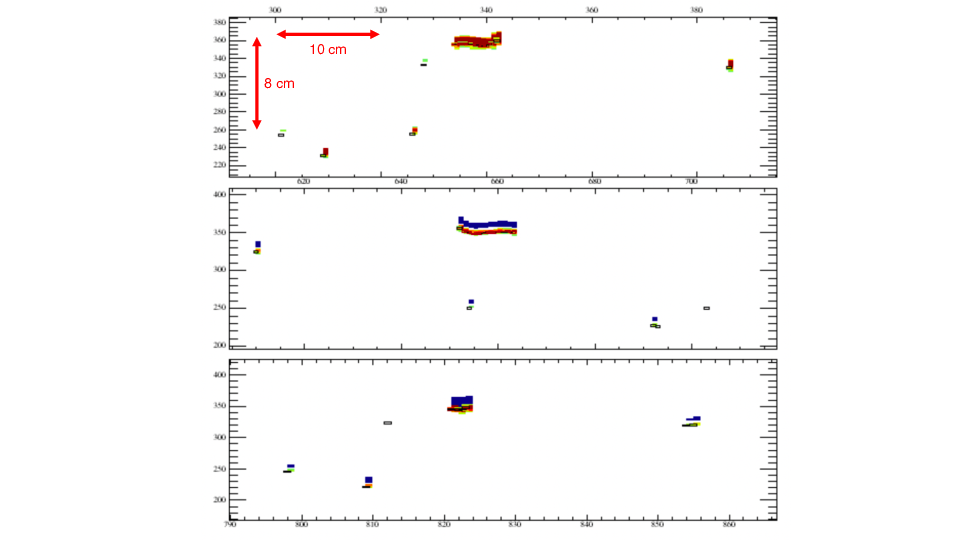
\includegraphics[width=\textwidth]{graphics/IntroFigures/nueCC_20-25MeV_event25_2.png} %\hskip 1 in
%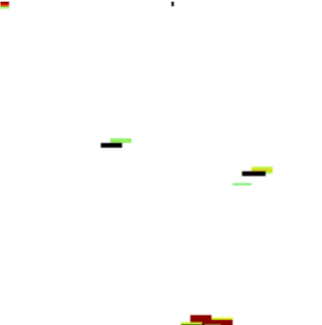
\includegraphics[height=0.5\textwidth]{graphics/IntroFigures/Fig_10b_Picture4.png}
\end{dunefigure}



Supernova candidates pose a unique problem for data acquisition and reconstruction.  \dword{snb} physics in DUNE is discussed in some detail in the far detector \dword{tdr}\cite{ Abi:2020evt}, reference \cite{Cuesta:2020dyj} and a dedicated paper \cite{DUNE:2020zfm} and only summarized here. 

\dword{dune} is uniquely sensitive to $\nu_e$ through the reaction $\nu_e + \hbox{Ar} \rightarrow e^- + \hbox{K}^*$ which leaves an electron trajectory that can be used to estimate the direction of the supernova.  Figure \ref{fig:SNrates} shows the expected neutrino interaction rates from supernovae as a function of their distance.
%The number of neutrino interactions actually detected depends on the physics of the supernova burst, oscillation physics and the minimum energy threshold achievable in the DUNE \dword{tpc} in the presencen of radiological backgrounds.

\hideme{HMS 3/2 added the missing figure}
\begin{dunefigure}
[Supernova rates in DUNE as a function of distance]
{fig:SNrates}
{Supernova rates in the DUNE detector  as a function of distance from the source from reference \cite{DUNE:2020zfm}.}
{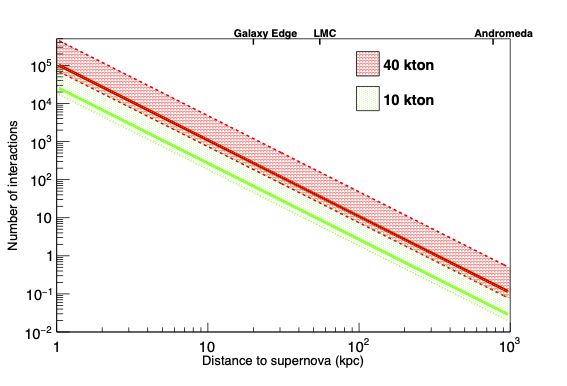
\includegraphics[width=0.9\textwidth]{graphics/IntroFigures/argon_sn.png}}
\end{dunefigure}

A classic core-collapse supernova 10\,kpc away would be expected to yield around 3,000  \dword{cc} electron neutrino interactions across four detector modules. \dword{snb} candidates will be quite different from beam interactions, having small interactions with energies in the 5-30\,MeV range spread across the full volume of the detector modules over many seconds, in contrast to the localized, coincident,  500-10,000\,MeV signature of beam neutrino interactions. These differences impose interesting requirements on the \dword{daq} and computing models for the experiment.  


\dword{snb} physics and its influence on neutrino emission are not fully understood and will result in significant modulations of the event rates for different neutrino types  over the few tens of seconds of the burst.  DUNE's fine-grained tracking should allow significant pointing power with the most optimistic scenario of four modules and high electron neutrino fraction yielding pointing resolutions of less than 5 degrees.   Figure \ref{fig:SNe} illustrates simulated signatures of \dword{snb} neutrino interactions in the far detector. The ability to produce a reasonably fast pointing signal would be extremely valuable to optical astronomers doing followup, especially if the supernova were in a region where dust masks the primary optical signal.   The need to be alert to supernovae and to quickly transfer and process the data imposes significant requirements on triggering, data transfer and reconstruction beyond those imposed by the %anne more regular 
beam-based oscillation physics. 
%For example, a compressed \dword{snb} readout of all four modules will be of order 184\,TB in size and take a minimum of four hrs to transfer over a 100\,Gbs network,  and then take of order 130,000 CPU-hrs for signal processing at present speeds.  If processing takes the same time as transfer, a peak of 30,000 cores would be needed. 

%%\subsection{Supernova \hideme{Schellman/Kirby - needed}}
%\todo{should this move to the introduction} 
%\cite{Cuesta:2020dy} % CHEP talk

%As noted in the introduction, the  \dword{dune} far detectors are sensitive to core-collapse supernovae.  References \cite{DUNE:2020zfm, Cuesta:2020dy} describe recent simulation studies of DUNE's sensitivity to core-collapse supernova signals in our Galaxy.

% \dword{dune} is uniquely sensitive to $\nu_e$ through the reaction $\nu_e + Ar \rightarrow e^- + K*$ which leaves an electron trajectory that can be used to estimate the direction of the supernova.  Figure \ref{fig:SNrates} shows the expected neutrino interaction rates from supernovae as a function of their distance.
% The number of neutrino interactions actually detected depends on the physics of the supernova burst, oscillation physics and the minimum energy threshold achievable in the DUNE \dword{tpc} in the presencen of radiological backgrounds. 

The \dword{tpc} and \dword{pd} detectors produce several signals of increasing precision.  First, scintillation light is detected by the photon detectors, yielding fast triggering information.  Trigger primitives based on a subset of the \dword{lartpc} information can also be searched for supernova signatures.  Finally a full detector readout can be mined for information across the full spatial and energy range of the detector over a period of up to 100 s.  Trigger information from the \dwords{pds} and trigger primitives is available quickly and would lead to a completed long readout of the full detector system in the event that a candidate \dword{snb} is detected. 

In reference \cite{DUNE:2020zfm} the performance and efficiency of fast triggering on scintillation light and \dword{tpc} hits are investigated.  Radiological and noise backgrounds are required to produce less than 1 false trigger/month. Both \dword{pd} and \dword{tpc} based triggers are sensitive relatively low numbers of interactions ($\sim10-25$) at acceptable background rates, yielding expected sensitivities out to the Large Magellanic cloud.

Once the trigger system has identified a potential \dword{snb} signal  the \dword{daq} then records information for 100 s, yielding 140 TB of uncompressed information for a \dword{hd} module and 180 TB for a \dword{vd} module.  These data must then be transferred offsite for processing with the full algorithms. 

%Information from \dword{dune} comes at three levels.  First,  fast identification of a supernova candidate, based on raw \dwprd{toc} and \dword{pd}  information, second, first-pass pattern recognition on a subset of the data which could provide pointing information on a time scale of seconds to hours and finally, full reconstruction of all information available down to the detector threshold in the few MeV range to exact maximal physics information from these extremely rare events. %Optimal use of this information requires 



Moving  320 TB (assuming the first 2 modules) of uncompressed data   from \dword{surf} to processing centers will require, at minimum, 6-7 hours with the planned 100Gbs network link.  This can be accelerated by implementing onboard data compression and may require upgrades to the network when the projected third and fourth modules come online.  The need to store up to 320 TB of data from a supernova candidate while also continuing normal data taking drives the size of local disk buffers at \dword{surf} and presumably required similar reserved or rapidly-preemptable space at the centers where the data would be processed. Our \dword{protodune} experience indicates that reconstruction of \dword{lartpc} data takes between 1 and 3 sec/MB of raw data on present day computing resources.  It will thus take of order 12,000-40,000 cores to perform a preliminary reconstruction the data as fast as it comes in. In principle, a significant fraction of the neutrino data could be processed  in the 2-4 hours before a supernova becomes visible at optical frequencies.

Other neutrino detectors worldwide will also be able to provide fast information but the \dword{dune} information will be unique in its sensitivity to electron neutrinos. 


% \hideme{HMS give up on this 
\subsection{Other phenomena -- Solar Neutrinos and Beyond-the-Standard-Model Processes} %\hideme{???-needed}}
There are multiple other measurements that can be made in  massive low background detectors such as the \dwords{fd}.  These are described in a recent White Paper \cite{Caratelli:2022llt}. These include detection of solar neutrinos and searches for \dword{bsm} processes such as neutron-anti-neutron oscillations.  Detection of these rare processes will require low radiological backgrounds and trigger systems capable of reading out the detector at rates low enough to remain well below a 30 Pb/year limit on data logging.  They will require recording the full waveforms, perhaps over a limited geographical region, to perform optimal signal extraction. In this document we concentrate on the oscillation, calibration and \dword{snb} scenarios as they are likely to dominate data rates in the near term.  
%\fixme{ Need someone to write about solar/BSM signature}}

%\todo{more test on the network and processing challenges}



\section{Near Detector \hideme{Junk/Muether - needs update}}

High-precision oscillation physics requires a \dword{nd} system to allow measurement of the unoscillated neutrino flux and %anne improved understanding of neutrino interaction physics. 
to provide improved understanding of neutrino interaction physics. 
The DUNE  collaboration is proposing a suite of near detectors optimized for these two goals. The proposed detectors are described in more detail in the Near Detector Conceptual Design Report \cite{DUNE:2021tad}.
 
 The \dword{nd}  will be located in an enclosure on the \dword{fnal} site 574\,meters from the target %anne and will be exposed to the DUNE 
 in the path of the neutrino beam.    Interaction rates per spill (at 0.83\,Hz) are expected to be very large, with 40-60 interactions per spill, including muons originating from interactions in material upstream of the fiducial volumes. Figure~\ref{fig:beamline} shows the beamline and location of the \dword{nd} on the \dword{fnal} site. There are three major subdetectors:
 A pixel readout %anne liquid argon detector
 \dword{lartpc}, \dword{ndlar}, is  the most upstream of the three subdetectors shown in Figure~\ref{fig:nd}, where the beam propagates  from right to left. Immediately downstream of \dword{ndlar} is a detector for characterizing muons exiting the \dword{ndlar}. This will initially be a magnetized steel range stack detector (TMS). A gaseous liquid argon detector, \dword{ndgar}, which serves %anne \dword{ndlar} 
 as  a muon spectrometer and allows more detailed study of neutrino interactions is planned for future operation when better control of neutrino interaction uncertainties is required. %anne that occur within its gas volume. 
 Beyond TMS/\dword{ndgar}, is the \dword{sand} component of the \dword{nd} that acts as a beam monitor. %Figure \ref{nd} shows the three \dword{nd} subdetectors in the near enclosure. 
Note that while the \dword{nd} will have the same DAQ timing window flexibility as the \dword{fd}, it is not foreseen that \dword{nd} physics goals will required the utilization of varied time windows for trigger records as compared with the \dword{fd}. %Kirby


 \begin{dunefigure}
[The neutrino beamline on the Fermilab site]
{fig:beamline} % Anne: label should have fig:
{The neutrino beamline on the \dword{fnal} site. The near detectors will be situated 574\,m from the target and 62\,m below grade.}
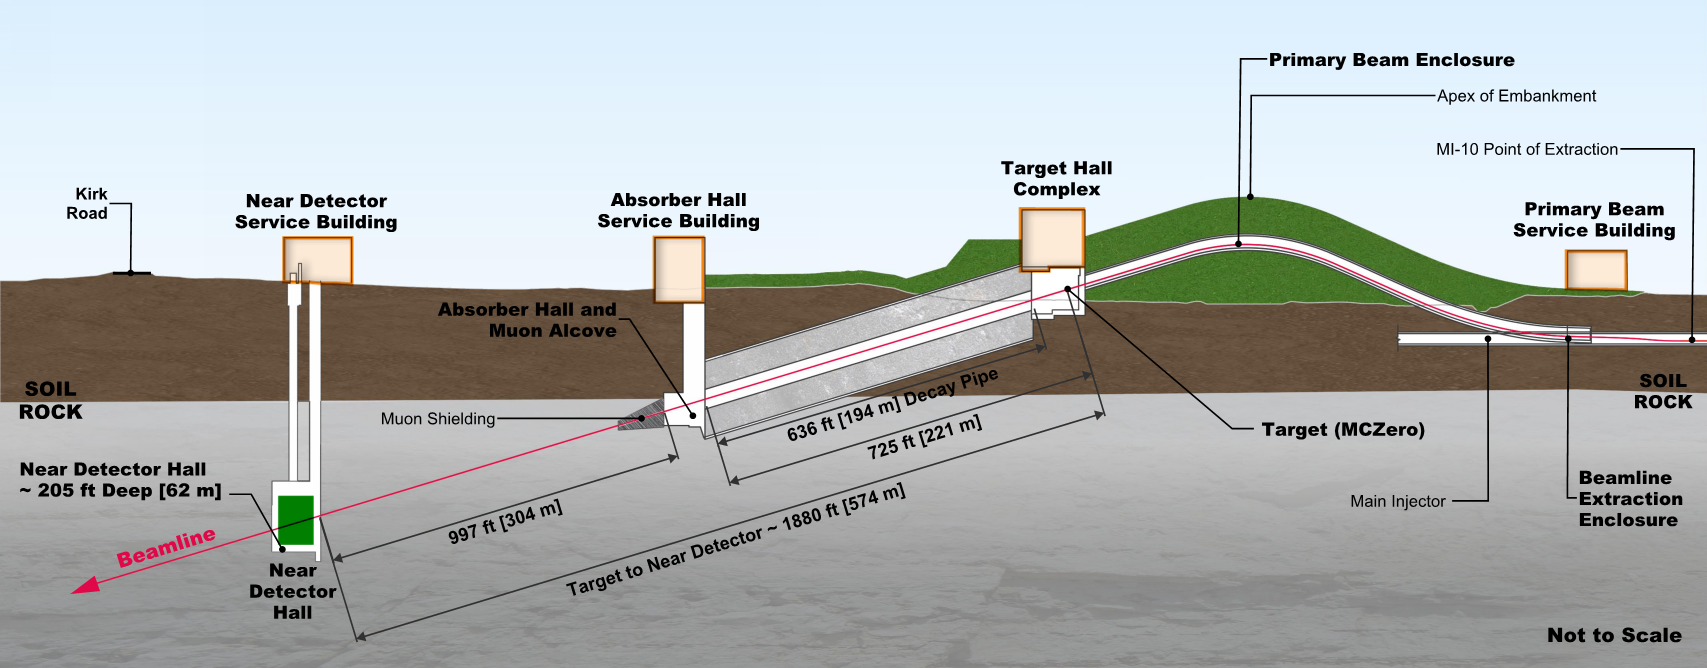
\includegraphics[height=0.3\textwidth]{graphics/IntroFigures/beamline-sideview.png}
\end{dunefigure}

 
 \begin{dunefigure}
[The ND systems in an on-axis configuration]
{fig:nd}
{The \dword{nd} systems in an on-axis configuration.  The beam enters from the lower right in this view. The \dword{sand} scintillating beam monitor remains at beam center while the pixel %anne ND-LAr TPC detector 
\dword{ndlar} and gaseous \dword{ndgar} \dword{tpc} detectors can be moved off-axis to make detailed studies of the neutrino flux at multiple angles.}
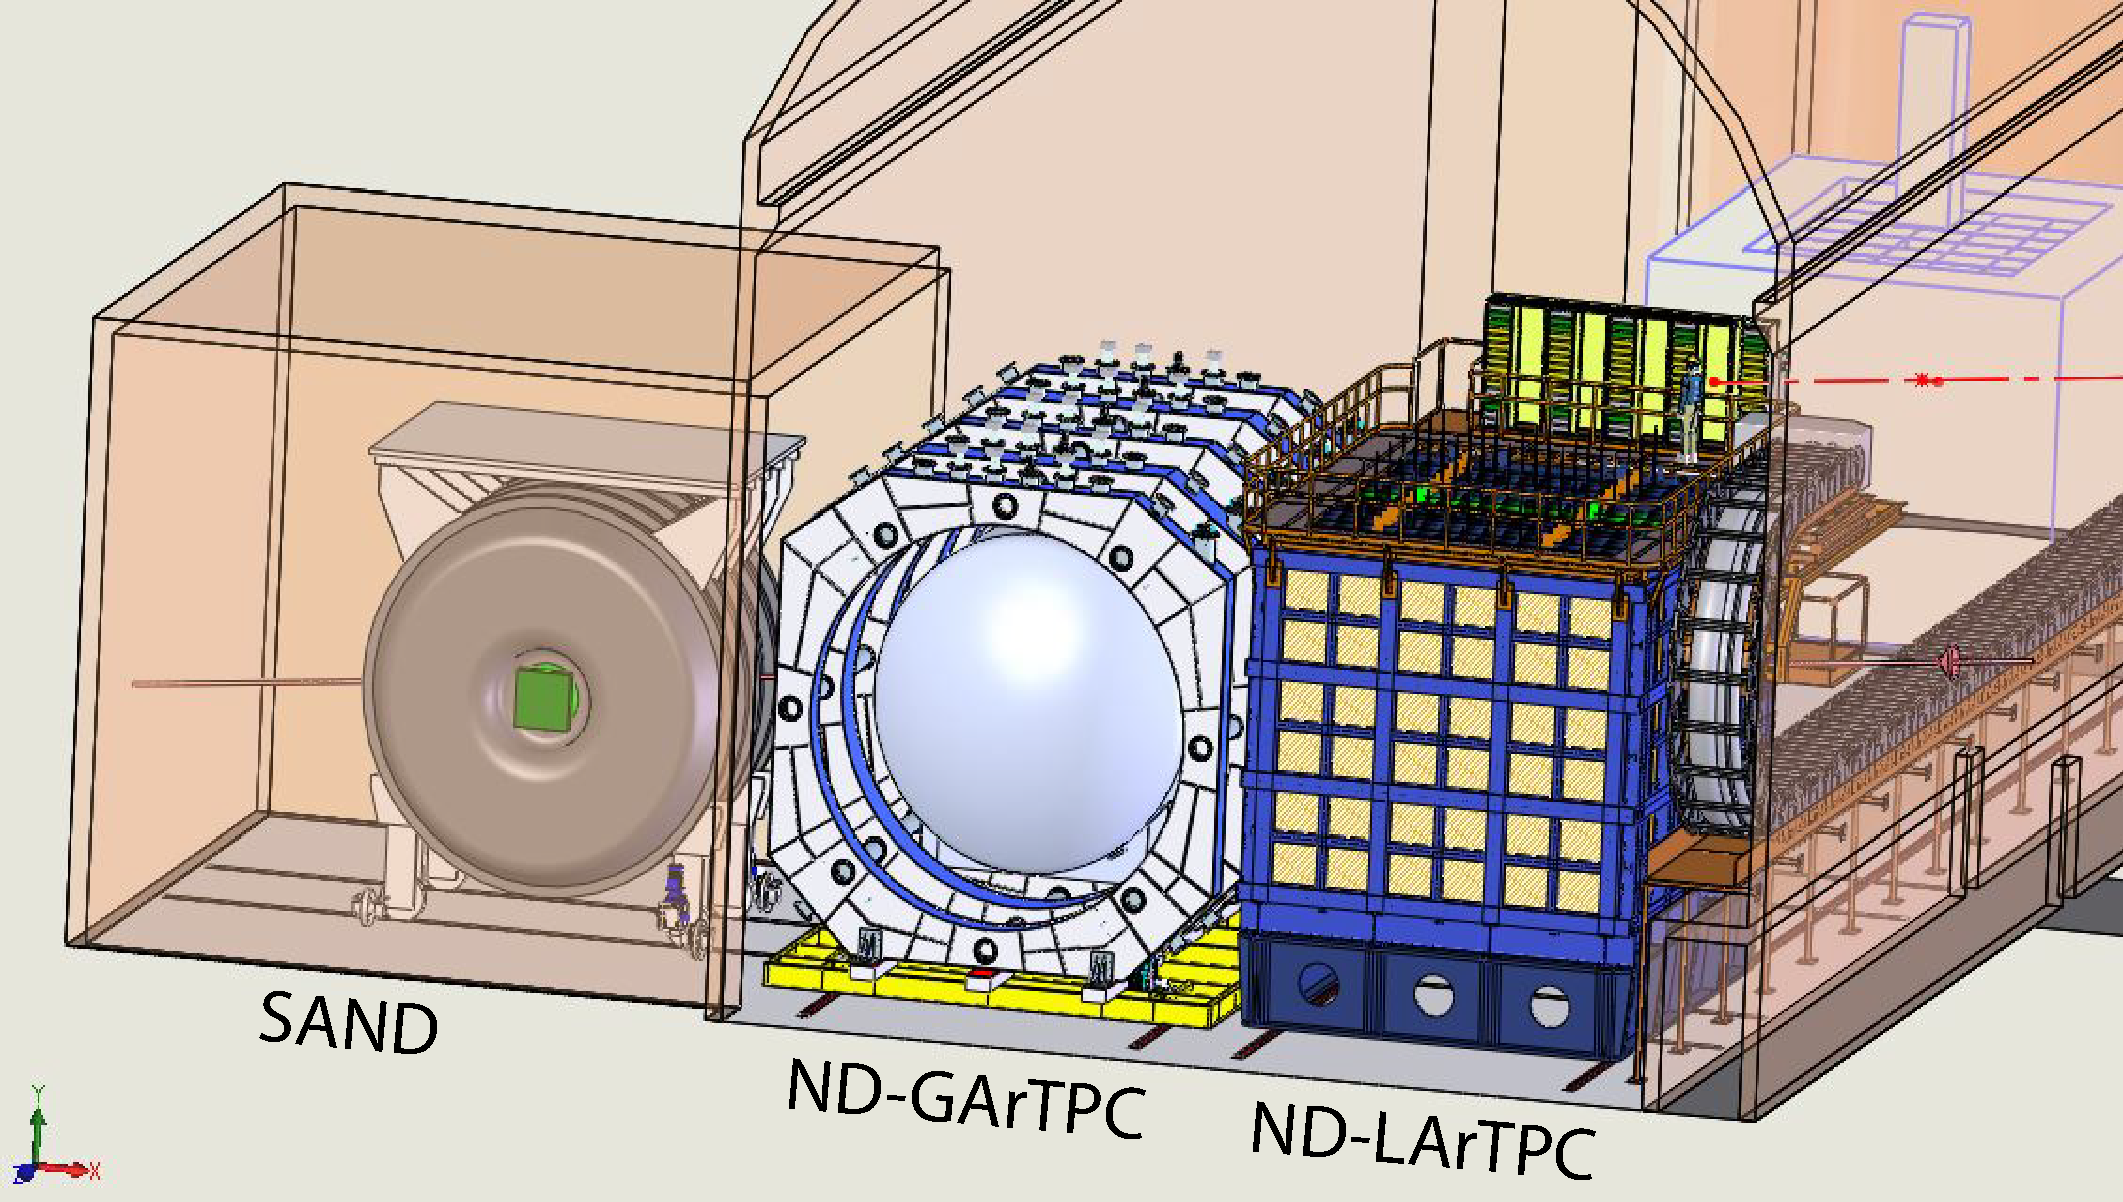
\includegraphics[height=0.5\textwidth]{graphics/IntroFigures/All3Detectors.pdf}
\end{dunefigure}

 \subsection{Pixel \dshort{lartpc} - \dshort{ndlar} \hideme{Muether - draft}}
 
 As the target material in the %anneDeep Underground Neutrino Experiment (DUNE) 
 far detector is \dword{lar}, optimal cancellation of systematic uncertainties between the near and far detectors requires that the near detector include a  \dword{lar} component to match the \dword{fd}.  However, at the intense neutrino flux and high event rate in the \dword{nd} region, occupancies will be too high to allow the \twod readout provided by conventional wire planes. A new \dword{arcube}  technology has been developed that allows pixelized charge readout and, along with modularity and highly capable light detection, provides unambiguous \threed imaging of  particle interactions.  The \dword{ndlar} component of the \dword{nd} is made up of a configuration of \dword{arcube}  \dwords{lartpc}  large enough to provide the required hadronic shower containment and statistics.  %The 5 m (along beam)×7 m (horizontal,  transverse to beam)×3 m (height), 67 t fiducial mass, of ND-LAr are optimized primarily for  hadronic containment under the assumption that ND-GAr will measure the sign and momentum  of downstream exiting muons. Figure 2.2 shows the arrangement of modules in the crystat for  ND-LAr.  Section 2.2 gives a discussion of the physics consideration
 
 The pixel \dword{lar} detector will have 12~million $3 \times 3$\,mm$^2$ pixel channels and $\sim$4200 \dword{pd} channels.  The \dword{lartpc} will read out only pulse times and integrals, in contrast to the far detector which reads out every time slice.  The \dwords{pd} will, however, read out complete wave-forms.   A total of 3\,MB of uncompressed data is anticipated per spill from the \dword{tpc} with 5\,MB from the \dwords{pd} leading to an estimate of 144\,TB/year for uncompressed in-spill data. Calibrations and cosmic ray data increase that data volume by around 20\%.

% For calibrations, 300 runs are assumed to be taken per year, each generating 10~GB of data, for the TPC, and a similar set of runs for the photon detectors.  These runs include pulser runs, laser runs, radioactive source runs, or other special-condition runs that require taking data outside of the regular spills.  Since they are not tied to the spill timing structure, they can be collected at higher trigger rates and take less time.

% In addition to the beam data, cosmic rays will contribute to the data volume.  For the \dword{ndlar} geometry in the ND hall, the anticipated rate
% of cosmic rays is 100~Hz.  If all cosmic ray data were collected, the data volume would be approximately 1~MB/sec.  The scenario considered here is to
% collect one spill's worth of cosmic ray data for every ten beam spills, for a data volume of 6.3 TB per year.  While the activity on the cosmic-ray triggers is expected to be much less than that on a beam spill, it is assumed that the cosmic-ray triggering will continue even when the beam is off.

% The TPC-only out-of-spill and calibration numbers have been scaled by 8/3 to account for photon detector data, assuming full waveform readout in these samples, yielding the same ratio as in-spill data and the same compression. 

\subsection{Near Detector Day One Muon Spectrometer (TMS) \hideme{Muether - draft}}
\label{sec:comp-dataestimates-mpd}

The TMS, a low-cost low-risk detector, will operate for the early part of the DUNE running when beam intensities are at their lowest and DUNE is not systematics limited. The TMS is a magnetized steel range stack (similar to MINOS \cite{minosNIM}) between ND-LAr and SAND.  The purpose of the TMS is to measure the momentum of 1 - 5 GeV muons that exit ND-LAr by range with a momentum precision comparable to the Far Detector (taken to be 4\%). The steel will be magnetized to identify the charge of muons it detects with better than 98\% accuracy. These metrics are designed to ensure the DUNE physics program will function for the first 2-3 years of TMS operations with no degradation to physics output.

The TMS is placed 8.2 m downstream from the ND-LAr (center to center) and centered 2.51 m below the origin in $y$. The TMS consist of 200 total layers of alternating layers made up of magnetized steel plates and scintillator bars. The first 40 layers of steel are 1.5 cm thick. The rear 60 layers of steel are 4 cm thick. There is a 4 cm gap between each steel layer.  The thin (thick) central steel is given a vertically oriented downward pointing field of 1.25 T (0.9 T), while the outer steel thin (thick) steel plates have their field pointing upwards with a strength of 1.5 T (1.0 T). The scintillator is implemented as a collection of 3.5~cm wide by 3~m tall by 1~cm thick vertical bars arranged into modules of 1.68 m wide. Four modules are placed side by side into a layer. These scintillator layers are replicated in the gap between steel layers.  

 

\subsection{Near Detector \dshort{gartpc} \hideme{Muether - draft}}
\label{sec:comp-dataestimates-gartpc}

The \dword{ndgar} is a magnetized detector system consisting of a high-pressure \dword{gartpc} surrounded by an \dword{ecal} and a muon system. The \dword{ndgar} measures the momentum and sign of charged particles exiting the \dword{ndlar}. In addition, for neutrino interactions occurring in the \dword{ndgar} itself, higher resolution and lower momentum thresholds can be achieved for charged particle tracks, leading to improved neutrino interaction models. This capability enables further constraints of systematic uncertainties for long-baseline neutrino  oscillation analyses.

The \dword{ndgar} is composed of 678,136 readout pads in the \dword{tpc}, and approximately 3~million channels in the \dword{ecal}.  Approximately one in five spills will generate an interaction in the \dword{gartpc}, but particles entering the gas from interactions in the \dword{ecal} will provide the bulk of the data volume.  The readout strategy will be similar to the \dword{lartpc}, with only time and integral recorded. A  data volume of 2\,MB of uncompressed data per spill is expected from the \dword{tpc}.  The calorimeter is expected to contribute approximately 1\,MB per spill of uncompressed data.

% For calibrations, 300 runs per year generating 10~GB of data per run are assumed for the TPC, and a similarly-sized set of calibration runs are assumed for the \dword{ecal}.  Cosmic rays are expected to be collected between spills and when the beam is off.

\subsection{SAND \hideme{Muether - draft}}
\label{sec:comp-dataestimates-sand}
%The 3rd detector subsystem is the \dword{sand}, a scintillator based monitor, consists of a 3-D pixelated scintillator detector, an electromagnetic calorimeter and XXX

The \dword{sand} component of the \dword{nd}'s primary function is the primary beam flux monitor.   \dword{sand} consists of an active scintillator target \dword{3dst} followed by a tracking system immersed in a solenoidal superconducting magnet  and  a $4\pi$ electromagnetic calorimeter.

\dword{sand}'s \dword{3dst} calorimeter component is composed of 11,520,000 $1\times 1\times 1$~cm$^3$ scintillating cubes, read out by 153,600 fibers.  There are expected to be approximately 2,160 hits per spill with a total of 0.13\,MB of data per spill.  The  \dword{ecal}~\cite{Adinolfi:2002zx} uses 4,850 \dwords{pmt}, with an estimated 5,500 total hits per spill or 33\,kB of packed data per spill.   The data volume from \dword{sand} is 4.3\,TB/year with these assumptions.  The amount of data from out-of-spill cosmic rays is estimated to be 20\% of that of the in-spill data, or approximately 1\,TB.  The data volume from \dword{sand} is significantly smaller than that from the \dword{ndlar} and the \dword{ndgar} due to the relative sizes of the three-dimensional tracking volumes and the segmentation choices.



% Test using \dword{tms}

%\subsection{Simulation challenges}

\section{Relation of Physics Goals to Offline Computing Challenges \hideme{Schellman-draft}}

The DUNE physics program drives several detector characteristics that pose novel computing challenges.  While the overall data volumes are smaller than those routinely handled by the large \dword{lhc} experiments, the remote detector site and unique physics goals present novel computing challenges. 

\begin{description}
\item{\bf Fine segmentation needed for electron-photon discrimination: \\}   The primary goal of the DUNE long baseline experiment is measurement of $\nu_\mu\rightarrow\nu_e$ and $\nubar_\mu\rightarrow\nubar_e$
oscillation probabilities for GeV scale accelerator neutrinos.   These oscillation probabilities are intrinsically low and sensitive to backgrounds where the neutral current process  $\nu_\mu+A\rightarrow\nu_\mu+\gamma/\pi^0+X$
produces a photon or $\pi^0$ meson that %anne fakes 
mimics an oscillation signal.  Fine detector segmentation is necessary to distinguish between these scenarios. Figure~\ref{fig:Argoneut} illustrates this capability. The need for sub-cm-level segmentation drives the technology choice of \dwords{lartpc} and %anne hence 
the number of channels.   
\item{\bf Low-energy thresholds for astrophysical neutrinos: \\}
Other important physics goals are the detection of astrophysical neutrinos from the sun, possible supernovae burst neutrinos, atmospheric cosmic rays and %physics beyond the standard model (BSM) 
\dword{bsm} signatures in the \dword{fd}.  Astrophysical neutrinos produce lower-energy signatures, in the 1-30\,MeV range. Extracting such signals, near the noise threshold of the detector and in the presence of radiological backgrounds, requires careful attention to signal processing and zero-suppression for the \dword{fd} \dword{tpc} and \dword{pd} wave forms.  The need to optimize the low-energy threshold drives our need to carefully record waveforms with minimal processing. 

\item{\bf Precise energy calibrations:\\}
An additional challenge in oscillation physics is the need for accurate energy calibration in order to fully %anne utilize 
exploit the energy spectrum of the reconstructed neutrinos to further constrain oscillation parameters. While \dword{lar} detectors have a reputation for stability, the large volumes, complex \efield configurations, liquid motion, and potential variations in electron lifetime and drift velocity make it necessary to have large calibration data samples that span the full \dword{fd} detector volume.  Large cosmic ray and artificial calibration samples will dominate the total data volumes from the \dword{fd}. 

\item{\bf Supernovae:\\}A %anne supernova 
\dfirst{snb} candidate will generate 320\,TB of (uncompressed) data across the first two modules. This means tens of thousands of data files produced over a 100\,s period. These data must be recorded at low energy threshold due to the expected interaction energy range, but must also be analyzed quickly and coherently in order to measure the time evolution of neutrino emissions, which carries invaluable information about the supernova process itself. In addition, if \dword{dune} can quickly analyze \dword{cc} interactions, we can provide pointing information to telescopes for optical followup.  %anne Supernova 
\dword{snb} physics drives the need for fast data transmission from the \dword{fd} to computing facilities and for robust tracking of data movement so that a full picture of the supernova interaction can be reassembled after signal processing.
As well, the drastically different time scale of \dword{snb} physics places requirements on the software framework. %Kirby

\item{\bf \dword{nd} integration: \\}
While the \dword{fd} %detectors 
modules produce large data volumes, the detectors themselves are reasonably simple, consisting of a small number of technologies and large numbers of repeating components.  The \dword{nd} is much more complex. 

The \dword{nd} use case is similar to other fixed target experiments such as \dword{sbnd} at \dword{fnal} and \dword{compass} at \dword{cern}.  The main computing challenge for the \dword{nd} will be integration of a large number of disparate detector technologies into a coherent whole. Here careful attention to simulation, detector geometry and configuration, and code management will be the major challenges. 

\item{\bf Analysis and parameter extraction:\\}
%ST changed four continents to five since we now have collaborators in Africa also
\dword{dune} has over one thousand collaborators spread across five continents. Those collaborators will want to analyze our data over several decades. Fortunately, once reconstruction has been done, neutrino interaction samples are generally simpler than event records at colliders and should %anne be analyzable locally. 
allow researchers to analyze them at their local institutions. However, final parameter extraction  using large numbers of nuisance parameters remains a computationally intense problem and will require significant resources
and efficient utilization of \dword{hpc} to quickly achieve final results. 



\end{description}

\section{Summary of Challenges \hideme{Schellman-draft}}

DUNE offline computing faces four major challenges, some of which are unique to DUNE and others shared widely by \dword{hep} experiments.  

\begin{description}
\item{\bf Large memory footprints -}  DUNE events, with multiple data objects consisting of  thousands of channels with thousands of time samples   present formidable challenges for reconstruction on typical \dword{hep} processing systems. Efficient processing of DUNE data will require careful attention to data formats and, likely, substantial redesign of the processing framework to allow sequential processing of chunks of data.  Chapters~\ref{ch:use} and~\ref{ch:fworks} describe the status of applications and frameworks. 

\item{\bf Storing and processing data on heterogeneous international  resources -} DUNE depends on the combined resources of the collaboration for large-scale storage and processing of data.   Tools for using shared resources ranging from small-scale clusters to dedicated \dword{hpc} systems need to be developed and maintained.   Fortunately, \dword{hep}, through the \dword{wlcg}, \dword{osg} and \dword{hsf}  has a well developed ecosystem of tools that allow reasonably transparent use of collaboration computing resources.  Chapters~\ref{ch:est}, \ref{ch:cm} and~\ref{ch:datamgmt} describe the data volumes, computing model and data management plans. 

\item{
\bf Machine learning - }  Use of machine learning techniques can greatly improve simulation, reconstruction and analysis of data. However, integration of \dword{ml} techniques into a software ecosystem of the size and complexity of a large \dword{hep} experiment requires substantial effort beyond the original demonstration.  How is the \dword{ml} trained?  What special data format or processing requirements are present? How is the algorithm versioned and preserved to ensure reproducibility?   Chapters~\ref{ch:use} and~\ref{ch:codemgmt} discuss the applications and management.

\item{\bf Keeping it all going -}  %anne There are a 
A large suite of activities, %anne that are 
while not necessarily novel, %anne but 
still need to be done over the full lifetime of the experiment.  These include database design and operations, security updates, code management, documentation, training and user support.   For example, the \dword{nd} presents few novel computing challenges in memory or CPU use but is highly complex in terms of the number of detector systems that must be integrated. Another example is the continuing evolution of operating systems and security requirements.  These require constant modifications to working systems to maintain operations.  A third activity is database design and maintenance. Here the problem is largely sociological, getting the attention of busy people to do database design and then %anne population and use. 
populate and use the official collaboration databases. This requires continual engagement with reluctant stakeholders. These issues are discussed throughout this document with special reference to databases, Chapter~\ref{ch:db}, authentication Chapter~\ref{ch:auth}, code management Chapter~\ref{ch:codemgmt} and training and documentation Chapter~\ref{ch:train}
\end{description}
A broad suite of use cases is discussed in Chapter~\ref{ch:use}.


%\hideme{\section{What is missing?}}

\end{document}